\documentclass{article}
\usepackage{physics}
\usepackage{amsmath}
\usepackage{graphicx}
\usepackage{authblk}
\usepackage{amsfonts}
\usepackage{esint}
\usepackage{bbold}
\usepackage{mathtools}
\usepackage{dsfont}
\usepackage{amsthm}
\usepackage{bbm}
\usepackage{amssymb}
\theoremstyle{definition}
\newtheorem{defn}{Definition}[section]
\newtheorem{prop}{Properties}[section]
\newtheorem{rmk}{Remark}[section]
\newtheorem{exmp}{Example}[section]
\newtheorem{prob}{Problem}[section]
\newtheorem{sln}{Solution}[section]
\newtheorem{thm}{Theorem}[section]
\newtheorem*{prob*}{Problem}
\newtheorem*{sln*}{Solution}
\usepackage{empheq}
\usepackage{tensor}



\usepackage{hyperref}
\usepackage{xcolor}
\hypersetup{
	colorlinks,
	linkcolor={black!50!black},
	citecolor={blue!50!black},
	urlcolor={blue!80!black}
}
%\usepackage{mathabx}

\newcommand{\R}{\mathbb{R}}

\newcommand{\F}{\mathcal{F}}
\newcommand{\p}{\partial}

\newcommand{\Arg}{\text{Arg}}

\newcommand{\f}[2]{\frac{#1}{#2}}

\newcommand{\G}{\mathcal{G}}
\newcommand{\C}{\mathbb{C}}
\newcommand{\Uni}{\mathcal{U}}

\newcommand{\V}{\mathbf{V}}
\newcommand{\W}{\mathbf{W}}
\newcommand{\Z}{\mathbf{Z}}
\newcommand{\Y}{\mathbf{Y}}
\newcommand{\U}{\mathbf{U}}
\newcommand{\X}{\mathbf{X}}

\newcommand*{\operp}{\perp\mkern-20.7mu\bigcirc}

\newcommand{\A}{\mathcal{A}}
\newcommand{\B}{\mathcal{B}}

\newcommand{\xpan}{\text{span}}

\newcommand{\lag}{\mathcal{L}}

\newcommand{\J}{\mathbf{J}}

\newcommand{\M}{\mathcal{M}}

\newcommand{\K}{\mathcal{K}}

\newcommand{\N}{\mathcal{N}}

\newcommand{\E}{\mathcal{E}}

\newcommand{\ima}{\text{Im}}
\newcommand{\lin}{\overset{\text{linear}}{\longrightarrow}}
\newcommand{\T}{\mathcal{T}}
\newcommand{\poly}{\mathbb{P}}
\newcommand{\s}{\mathcal{S}}

\newcommand{\jor}{\mathcal{J}}
\newcommand{\FF}{\mathfrak{F}}
\newcommand{\LL}{\mathfrak{L}}
\newcommand{\lat}{\mathfrak{Lat}}

\newcommand{\gives}{\rotatebox[origin=c]{180}{$\Rsh$}	}

\newcommand{\la}{\langle}
\newcommand{\ra}{\rangle}

\newcommand{\lp}{\left(}
\newcommand{\rp}{\right)}

\newcommand{\lb}{\left[}
\newcommand{\rb}{\right]}


\newcommand{\nn}{\nonumber}

\newcommand{\id}{\mathcal{I}}

\newcommand{\bigzero}{\mbox{\normalfont\Large\bfseries 0}}
\newcommand{\rvline}{\hspace*{-\arraycolsep}\vline\hspace*{-\arraycolsep}}



\usepackage{subfig}
\usepackage{listings}
\captionsetup[lstlisting]{margin=0cm,format=hang,font=small,format=plain,labelfont={bf,up},textfont={it}}
\renewcommand*{\lstlistingname}{Code \textcolor{violet}{\textsl{Mathematica}}}
\definecolor{gris245}{RGB}{245,245,245}
\definecolor{olive}{RGB}{50,140,50}
\definecolor{brun}{RGB}{175,100,80}
\lstset{
	tabsize=4,
	frame=single,
	language=mathematica,
	basicstyle=\scriptsize\ttfamily,
	keywordstyle=\color{black},
	backgroundcolor=\color{gris245},
	commentstyle=\color{gray},
	showstringspaces=false,
	emph={
		r1,
		r2,
		epsilon,epsilon_,
		Newton,Newton_
	},emphstyle={\color{olive}},
	emph={[2]
		L,
		CouleurCourbe,
		PotentielEffectif,
		IdCourbe,
		Courbe
	},emphstyle={[2]\color{blue}},
	emph={[3]r,r_,n,n_},emphstyle={[3]\color{magenta}}
}


\begin{document}
	\begin{titlepage}\centering
		\clearpage
		\title{\textsc{\bf{Introductory Topics in \\ Complex Analysis}}}
		\author{\bigskip Huan Q. Bui}
		 \affil{Colby College\\$\,$\\ PHYSICS \& MATHEMATICS\\ Statistics \\$\,$\\Class of 2021\\}
		\date{\today}
		\maketitle
		\thispagestyle{empty}
	\end{titlepage}




\newpage
\tableofcontents
\newpage



\section{de Moivre's Formula}

\begin{align}
(\cos\theta + \sin\theta)^n = \cos n \theta + i\sin n \theta.
\end{align}

\section{Roots \& Things}

All roots of $z = r_0 e^{i\theta}$ are of the form
\begin{align}
z_r = r_0^{1/n}\exp\lp \f{\theta_0}{n} + \f{2k \pi}{n} \rp
\end{align}
where $k = 0,1,2,\dots$


\section{Regions of the Complex Plane}

\noindent $\spadesuit$ The $\epsilon$-neighborhood of $z_0$ is the set of points
\begin{align}
\B_\epsilon (z_0) := \{ z\in \C : \abs{z - z_0} < \epsilon \}.
\end{align}

\noindent $\spadesuit$ The deleted $\epsilon$-neighborhood (nbh) of $z_0$ is the set
\begin{align}
\B_\epsilon(z_0) \setminus \{z_0\} = \{ z\in \C : 0 < \abs{z - z_0} < \epsilon \}.
\end{align}

\noindent$\spadesuit$ $z_0$ is an interior point of $S \subset \C$ if some $\epsilon$-nbh is completely contained in $S$, i.e.,
\begin{align}
\exists \B_\epsilon(z_0) \text{ s.t. } \B_\epsilon(z_0) \subset S.
\end{align}


\noindent $\spadesuit$ $z_0$ is an exterior point of $S$ if $\exists \B_\epsilon(z_0)$ which does not intersect $S$.\\

\noindent $\spadesuit$ If $z_0$ is neither an interior nor an exterior point of $S$ then it is called a boundary point of $S$. The set of boundary points of $S$ is called the boundary of $S$.\\

\noindent $\spadesuit$ $z_0$ is a boundary point of $S \iff \forall \epsilon> 0, \B_\epsilon(z_0)$ contains at least one point in $S$ and at least one point in $S^c$.\\

\noindent $\spadesuit$ A set $\mathcal{O}$ is called open if it contains none of its boundary points. \\

\noindent $\spadesuit$ A set $C$ is called closed if it contains all of its boundary points. \\

\noindent $\spadesuit$ The closure of a set $S$ is the set $\text{cl}(S) = S \cup \p S$.\\

\noindent $\spadesuit$ Let $\mathcal{O} \subset \C$. $\mathcal{O}$ is open $\iff$ $\forall z \in \mathcal{O}, \exists \epsilon > 0, \B_\epsilon(z) \subset \mathcal{O}$.  \\

\noindent $\spadesuit$ A set $S$ is called path connected if $\forall z_1,z_2 \in S$, there exists a continuous function $\gamma: [0,1] \to \C$ such that $\gamma(0) = z_1, \gamma(1) = z_2$ and $\gamma(t) \in S \forall t \in [0,1]$.\\

\noindent $\spadesuit$ A set $S$ is bounded if $\exists R > 0$ such that $S \subset \B_R(0)$.\\

\noindent $\spadesuit$ A point $z_0$ is called an accumulation point of a set $S$ if $\forall \epsilon > 0$,
\begin{align}
\B_\epsilon(z_0)\setminus\{z_0\} \cap S \neq \emptyset,
\end{align} 
i.e. every deleted nbh of $z_0$ contains at least an element of $S$. \\

\noindent $\spadesuit$ A set is closed if and only if it contains all of its accumulation points.




\section{Limits}



\noindent $\spadesuit$ Let $f$ be a function defined on some punctured nbh of $z_0$. We say that the limit of $f$ is $w_0$ as $z$ approaches $z_0$ and write 
\begin{align}
\lim_{z\to z_0} f(z) = w_0
\end{align}
if $\forall \epsilon > 0, \exists \delta  > 0$ such that
\begin{align}
\abs{f(z) - w_0} < \epsilon \text{ whenever } 0 < \abs{z- z_0} < \delta
\end{align}
for $z \in \text{dom}(f)$. \\

\noindent $\spadesuit$ \textbf{Proposition:} Limits are unique.

\begin{proof}
	Assume that 
	\begin{align}
	&\lim_{z\to z_0} f(z) = w_0\nn\\
	&\lim_{z\to z_0} f(z) = w_1.
	\end{align}
	Given $\epsilon > 0$, choose $\delta_0, \delta_1 > 0$ such that
	\begin{align}
	\abs{f(z) - w_0} < \epsilon \text{ whenever } 0 < \abs{z- z_0} < \delta_0\nn\\
	\abs{f(z) - w_1} < \epsilon \text{ whenever } 0 < \abs{z- z_0} < \delta_1.
	\end{align}
	Consider $\delta = \min\{\delta_0, \delta_1\}$. Then, we have for some $z$ such that $0 < \abs{z - z_0} < \delta$,
	\begin{align}
	\abs{f(z) - w_0} < \epsilon \text{ and } \abs{f(z) - w_1} < \epsilon.
	\end{align}
	For this particular $z$, 
	\begin{align}
	\abs{w_0 - w_1} &= \abs{f(z) - w_0 - f(z) + w_1}\nn\\
	&\leq \abs{f(z) - w_0} + \abs{f(z) - w_1}\nn\\
	&< \epsilon + \epsilon \nn\\
	&= 2\epsilon.
	\end{align}
	So, for any $\epsilon > 0, \abs{w_1 - w_0} < 2\epsilon$. This means $w_0 = w_1$.
\end{proof}



\section{Limits obtained via an admissible path}

If $\lim_{z \to z_0} f(z) = w_0$, then given any continuous function $\gamma$ satisfying
\begin{enumerate}
	\item $\gamma: [0,1] \to \R^2 \equiv \C$ is continuous
	\item $\gamma(t) \neq z_0 \forall t > 0$, $\gamma(t) \in \text{dom}(f) \forall t > 0$
	\item $\gamma(0) = z_0$
\end{enumerate}
then $\lim_{t \to 0^+} f(\gamma(t)) = w_0$. Any path satisfying the three conditions above is said to be admissible for $f$ near $z_0$, or simply admissible. 

\section{Existence of Limits}

If given any two admissible paths $\gamma_0, \gamma_1$ we have
\begin{align}
\lim_{t \to 0^+} f(\gamma_0(t)) \neq \lim_{t \to 0^+}f(\gamma_1(t))
\end{align}
then $\lim_{z \to z_0} f(z)$ does not exist. 


\section{Connect to multi-variable calculus}

Suppose that $f(z) = u(x,y) + iv(x,y)$ and $z_0 = x_0 + iy_0$. Then 
\begin{align}
\lim_{z \to z_0} f(z) = w_0 = a_0 + ib_0
\iff
\begin{cases}
\lim_{(x,y)\to(x_0,y_0)}u(x,y) = a_0 \\ \lim_{(x,y)\to(x_0,y_0)}v(x,y) = b_0
\end{cases}
\end{align} 

\section{Limit facts}


Suppose that $\lim_{z \to z_0} f(z) = w_0$ and $\lim_{z \to z_0} F(z) = W_0$, then 
\begin{enumerate}
	\item $\lim_{z \to z_0} f(z) + F(z) = w_0 + W_0$.
	
	\item $\lim_{z \to z_0} f(z)F(z) = w_0 W_0$.
	
	\item If $W_0 \neq 0$ then $\lim_{z \to z_0} f(z)/F(z) = w_0 / W_0$.
\end{enumerate}


\begin{proof}
	We will prove the second statement. Let $z_0 = x_0 + iy_0$ and $f(z) = u + iv$ and $F(z) = U + iV$. Then
	\begin{align}
	f(z) F(z) = (uU - vV) + i (uV + vU).
	\end{align}
	Since the limits of $f,F$ at $z_0$ are given, we have
	\begin{align}
	&\lim_{(x,y)\to(x_0,y_0)} u = u_0\nn\\
	&\lim_{(x,y)\to(x_0,y_0)} v = U_0\nn\\
	&\lim_{(x,y)\to(x_0,y_0)} U = v_0\nn\\
	&\lim_{(x,y)\to(x_0,y_0)} V = V_0.
	\end{align} 
	Applying to the algebra of limits for $\R^2 \to \R$, we have
	\begin{align}
	\lim_{(x,y)\to(x_0,y_0)} (uU - vV) = u_0 U_0 - v_0V_0 = \Re(w_0 W_0).
	\end{align}
	Similarly,
	\begin{align}
	\lim_{(x,y)\to(x_0,y_0)} (uV + vU) = u_0 V_0 + v_0U_0 = \Im(w_0 W_0).
	\end{align}
	So, by the previous theorem, $\lim_{z \to z_0} f(z)F(z) = w_0W_0$.
\end{proof}




\section{$\epsilon$-neighborhood of $\infty$}


\noindent $\spadesuit$ Given $\epsilon> 0$, we call the set $\B_\epsilon(\infty) = \{ z \in \C : \abs{z} > 1\epsilon \}$ the $\epsilon$-nbh of $\infty$. \\

\noindent $\spadesuit$ Given $z_0 \in \C$ and $f$ defined on a nbh of $z_0$, we say that the limit of $f$ as $z\to z_0$ is $\infty$ and write
\begin{align}
\lim_{z \to z_0} f = \infty
\end{align}
if $\forall \epsilon > 0, \delta > 0$ s.t. $f(z) \in \B_\epsilon(\infty)$ whenever $z \in \text{dom}(f)$ and $z\in \delta-$nbh of $z_0$, i.e., $\forall \epsilon > 0, \exists \delta>0$ s.t. $\abs{f(z)} > 1/\epsilon$ whenever $0 < \abs{z-z_0} < \delta$.\\

\noindent $\spadesuit$ Additionally, we say $\lim_{z\to\infty} f(z) = w_0$ for $w_0 \in \C$ if $\forall \epsilon > 0,\exists \delta >0 $ s.t. $f(z)$ lines in the $\epsilon$-nbh of $w_0$ whenever $z\in$ the $\delta$-nbh of $\infty$, i.e., $\forall \epsilon > 0, \exists \delta >0 $ s.t. $\abs{f(z) - w_0} < \epsilon$ whenever $\abs{z} > 1/\delta$.\\

\noindent $\spadesuit$ Further, we say that the limit of $f$ as $z \to \infty$ is $\infty$ if $\forall \epsilon > 0, \exists \B_\delta(\infty)$ s.t. $f(z) \in \B_\epsilon(\infty)$ whenever $z\in \B_\delta(\infty)$. 


\section{Limit facts involving $\infty$}

Let $z_0, w_0 \in \C$, then 
\begin{align}
\lim_{z \to z_0} f(z) =\infty &\iff \lim_{z \to z_0}\f{1}{f(z)} = 0.\nn\\
\lim_{z\to\infty} f(z) = w_0 &\iff \lim_{z\to 0} f\lp \f{1}{z} \rp = w_0.\nn\\
\lim_{z\to\infty} f(z) = \infty &\iff \lim_{z\to 0} \f{1}{f\lp \f{1}{z}\rp} = 0.
\end{align}


\begin{proof}
	We will prove (3). Suppose that $\lim_{z\to\infty} f(z) = \infty$. Let $\epsilon > 0$ be given. Then $\exists \delta > 0$ s.t. $\abs{f(z)} > 1/\epsilon$ whenever $\abs{z} > 1/\delta$. Then $1/\abs{f(z)} < \epsilon$ whenever $\abs{z} > 1/\delta \iff \abs{w} = 1/\abs{z} < \delta$. Thus, for any $0 < \abs{w} < \delta$, we have that 
	\begin{align}
	\abs{\f{1}{f(1/w)}} = \f{1}{\abs{f(z)}} < \epsilon
	\end{align}
	as long as $w = 1/z$, i.e., $\forall \epsilon> 0, \exists \delta > 0$ s.t. $\abs{1 / f(1/z)} < \epsilon$ whenever $\abs{z} < \delta$. The converse is gotten by reversing the steps. 
\end{proof}



\section{Continuity \& 3 Theorems}

\noindent $\spadesuit$Let $f$ be defined on a full nbh of $z_0$. We say that $f$ is continuous at $z_0$ if the following hold:
\begin{enumerate}
	\item $\lim_{z \to z_0} f(z)$ exists. 
	\item $f(z_0)$ exists. 
	\item $\lim_{z \to z_0} f(z) = f(z_0)$. 
\end{enumerate}


\noindent $\spadesuit$ \underline{Compositions of continuous functions}: Suppose that $f$ is continuous at $z_0$ and $g$ is continuous at $f(z_0) = w_0$ then $g\circ f(z_0)$ is continuous at $z_0$. 

\begin{proof}
	Let $\epsilon > 0$ be given, then $\exists \gamma > 0$ s.t. $\abs{g(w) - g(w_0)} < \epsilon  $ whenever $\abs{w - w_0} < \gamma$. Given this $\gamma, \exists \delta > 0$ s.t. $\abs{f(z) - f(z_0)} < \gamma$ whenever $\abs{z -z_0} < \delta$. So, whenever $\abs{z - z_0} < \delta$,  $\abs{f(z) - f(z_0)} < \gamma$ and so $\abs{g(w) - g(w_0)} < \epsilon$. 
\end{proof}


\noindent $\spadesuit$ \underline{If a continuous function is nonzero at a point then it is nonzero near that point}: Suppose that $f$ is continuous at $z_0$ and $\abs{f(z_0)} \neq 0, \exists \delta > 0$ such that $f(z) \neq 0 \forall z \in \B_\delta(z_0)$.


\begin{proof}
	Choose $\epsilon = \abs{f(z_0)/2} > 0$. Then $\exists \delta > 0$ such that $\abs{f(z) - f(z_0)} < \epsilon = \abs{f(z_0)/2} \forall \abs{z - z_0 } < \delta$. Then, for  all such $z$, we have that
	\begin{align}
	\abs{f(z_0)} &= \abs{f(z_0) + f(z) - f(z)} \nn\\
	&\leq \abs{f(z_0) - f(z)} + \abs{f(z)}\nn\\
	&\leq \f{\abs{f(z_0)}}{2} + \abs{f(z)}.
	\end{align}
	So, $\forall z\in \B_\delta(z_0)$, we have $\abs{f(z_0)}/2 \leq \abs{f(z)}$. 
\end{proof}




\noindent $\spadesuit$ \underline{Continuous functions on a closed and bounded set is bounded}: Let $R$ be a closed and bounded subset of the complex plane. Let $f$ be continuous on $R$. Then $\exists M \geq 0$ such that
\begin{align}
\abs{f(z) } \leq M \forall z \in R
\end{align}
and $\exists z_0 \in R$ at which $\abs{f(z_0)} = M$. 



\section{Differentiability}


\noindent $\spadesuit$Let $f$ be defined in a nbh of $z_0$. The derivative of $f$ at $z_0$ is the limit
\begin{align}
f'(z_0) = \lim_{z \to z_0}\f{f(z) - f(z_0)}{z - z_0}
\end{align}
and it is defined whenever this limit exists. When this limit exists, we say $f$ is differentiable at $z_0$.\\

\noindent $\spadesuit$ If $f$ is differentiable at $z_0$, it is continuous at $z_0$. 

\begin{proof}
	Since the limit of the difference quotient exists,
	\begin{align}
	\lim_{z\to z_0} f(z) - f(z_0) &= \lim_{z\to z_0}\f{f(z) - f(z_0)}{z - z_0}(z- z_0)\nn\\
	&= \lim_{z\to z_0} \f{f(z) - f(z_0)}{z - z_0}\lim_{z \to z_0}(z - z_0)\nn\\
	&= f'(z_0)\cdot 0\nn\\
	&= 0.
	\end{align}
	Thus, $\lim_{z\to z_0} f(z) = f(z_0)$, and so $f$ is continuous at $z_0$. 
\end{proof}


\section{Differentiability Facts}

Let $f,g$ be differentiable at $z_0$ then 
\begin{align}
\begin{cases}
D_z (f+g)(z_0) = f'(z_0) + g'(z_0)\nn\\
D_z cf(z_0) = cf'(z_0)\nn\\
D_z f(z_0)g(z_0) = f'(z_0)g(z_0) + f(z_0)g'(z_0).
\end{cases}
\end{align}
If, additionally, $g(z_0) \neq 0$, then $f/g$ is differentiable at $z_0$ and
\begin{align}
D_z \f{f}{g}(z_0) = \f{f'(z_0)g(z_0) - f(z_0) g'(z_0)}{g^2(z_0)}.
\end{align}

\begin{proof}
	We shall prove the product rule:
	\begin{align}
	&\lim_{\Delta z \to 0} \f{f(z_0 + \Delta z)g(z_0 + \Delta z) - f(z_0)g(z_0)}{\Delta z}\nn\\
	= &\lim_{\Delta z \to 0}\f{1}{\Delta z}\lb (f(z_0 + \Delta z) - f(z_0) )g(z_0 + \Delta z) + f(z_0)g(z_0 + \Delta z) - f(z_0)g(z_0) \rb\nn\\
	= &\lim_{\Delta z \to 0}\f{1}{\Delta z} \lb \Delta f g(z_0 + \Delta z) + f(z_0)\Delta g \rb\nn\\
	= &g(z_0)f'(z_0) + g'(z_0)f(z_0),
	\end{align}
	where $g(z_0 + \Delta z)$ exists by continuity. 
\end{proof}

\section{The Chain Rule}

Let $f$ be differentiable at $z_0$ and $g$ be differentiable at $w_0 = f(z_0)$. Then $F(z) = g\circ f(z) = g(f(z))$ is differentiable at $z_0$ and $F'(z_0) \equiv D_z g\circ f(z_0) = g'(f(z_0))f'(z_0)$.


\begin{proof}
	On a nbh of $w_0$, define $\phi: N \to \C$ by 
	\begin{align}
	\phi(w) = \begin{cases}
	\f{g(w) - g(w_0)}{w - w_0} - g'(w_0) \quad w \neq w_0\\
	0 \quad w = w_0
	\end{cases}.
	\end{align}
	Observe that because $g$ is differentiable, $\lim_{w\to w_0}\phi(w) = 0$. It follows that $\phi$ is continuous on its domain. Also, for $w \in N$, 
	\begin{align}
	(w - w_0)\phi(w) = (g(w) - g(w_0)) - g'(w_0)(w - w_0).
	\end{align}
	Given the continuity of $f$ at $z_0$, we can choose $\delta > 0$ such that for $z \in \B_\delta(z_0)$ we have $f(z) = w \in N = \B_\epsilon(w_0)$ because
	\begin{align}
	\abs{f(z) - f(z_0)} = \abs{w - w_0} < \epsilon 
	\end{align}
	whenever $\abs{z - z_0} < \delta$. So, $\forall z \in \B_\delta(z_0)$, we have that $\phi(f(z))$ makes sense. Also, for these values of $z \neq z_0$,
	\begin{align}
	\f{F(z) - F(z_0)}{z - z_0} &= \f{g(f(z)) - g(f(z_0))}{z - z_0} \nn\\
	&= \f{g(w) - g(w_0)}{z - z_0} \nn\\
	&= \f{(w - w_0)\phi(w) + g'(w_0)(w - w_0)}{z  - z_0}\nn\\
	&= \f{(f(z) - f(z_0))\phi(f(z)) + g'(f(z_0))(f(z) - f(z_0))}{z  - z_0}.
	\end{align}
	Because $\phi(f(z))$ is continuous, $g'(z_0)$ is simply a constant, and $f$ is differentiable at $z_0$, we can easily see that
	\begin{align}
	\lim_{z \to z_0} \f{F(z) - F(z_0)}{z - z_0} &= f'(z_0)\phi(f(z_0)) + g'(f(z_0))f'(z_0).
	\end{align}
	But $\phi(f(z_0)) = \phi(w_0) = 0$ by definition, so we have
	\begin{align}
	F'(z_0) = g'(f(z_0))f'(z_0).
	\end{align}
\end{proof}


\section{The Cauchy-Riemann Equations}

Let $f(z) = u(x,y) + iv(x,y)$ be defined on a nbh of $z_0 = x_0 + iy_0$. Suppose that 
\begin{enumerate}
	\item $u,v$ have partial derivative on a nbh of $z_0$.
	\item All first order partial derivative are continuous on this nbh of $z_0$ and the C-R equations:
	\begin{align}
	u_x(x_0,y_0) = v_y(x_0,y_0);\quad u_y(x_0,y_0) = -v_x(x_0,y_0)
	\end{align}
	are satisfied.
\end{enumerate}
Then $f$ is differentiable at $z_0$ and
\begin{align}
f'(z_0) = u_x(x_0,y_0) + iv(x_0,y_0).
\end{align}


\begin{proof}
	The proof is not that bad, but it is quite technical. So I won't try to reproduce it here.
\end{proof}


\section{Analytic Functions: Differentiable on a Ball}

\noindent $\spadesuit$ A function $f$ is analytic at a point $z \in \C$ if it is differentiable on same nbh f $z_0$, i.e., at every point in $\B_\delta(z_0)$ for some $\delta > 0$.\\

\noindent $\spadesuit$ $f$ is said to be analytic on an open set $\mathcal{O}$ if it is analytic at each $z\in \mathcal{O}$.\\

\noindent $\spadesuit$ If $f$ is analytic on a set $S$, we say it is analytic on an open set $\mathcal{O} \subset S$. \\

\noindent $\spadesuit$ Vocabulary: Analytic $\equiv$ Holomorphic.\\

\noindent $\spadesuit$ A function $f$ is said to be entire if it is analytic on $\C$.

\noindent $\spadesuit$ If $z_0 \in \C$ is such that $f$ is analytic at every point in a nbh centered at $z_0$ but not at $z_0$ (i.e., analytic on $\B_\delta(z_0)\setminus \{z_0\}$) we say $z_0$ is a singular point for $f$. \\

\noindent $\spadesuit$ Suppose $f,g$ are analytic on an open set $\mathcal{O}$ then $f\pm g, fg$ are also analytic on $\mathcal{O}$. If $g(z) \neq 0 \forall z \in \mathcal{O}$ then $f/g$ is also analytic on $\mathcal{O}$. \\

\noindent $\spadesuit$ The set of analytic functions on an open set $\mathcal{O}$ form a commutative ring, denoted $\text{Hol}(\mathcal{O})$.


\section{Analytic Functions: Familiar, but Weird}

Suppose $\mathcal{D}$ is a domain (open, nonempty, path connected) and $f$ is analytic on $\mathcal{D}$. If $f'(z) =0 \forall z \in \mathcal{D}$ then $f$ is constant on $\mathcal{D}$. 

\begin{proof}
	Given $z_0, z_1 \in \mathcal{D}, \exists$ a path $\gamma(t) : [0,1] \to \mathcal{D}$ such that $\gamma(0) = z_0, \gamma(1) = z_1$, and $\gamma$ is a continuous. Next, consider $h(t) = \Re(f\circ \gamma(t)) = u(\gamma(t))$, where $f = u+ iv$. By C-R, we have that $f = u+ iv$ with $u,v$ both differentiable. And so $h(t)$ is differentiable on $[0,1]$, and by the mulvar chain rule
	\begin{align}
	h'(t) = u_x(\gamma(t)) \gamma_1'(t) + u_y(\gamma(t))\gamma_2'(t)
	\end{align}
	with $\gamma(t) = (\gamma_1(t), \gamma_2(t)) \forall t \in [0,1]$. By MVT, $\exists c \in (0,1)$ s.t.
	\begin{align}
	h(1) - h(0) &= h'(c)(1-0)\nn\\
	&= h'(c)\nn\\
	&= u_x(\gamma(c))\gamma_1'(c) + u_y(\gamma(c))\gamma_2'(c) \nn\\
	&= u_x(\gamma(c))\gamma_1'(c) - v_x(\gamma(c))\gamma_2'(c)
	\end{align}
	where the last equality follows from C-R. But we also know that $f' = u_x + iv_x = 0 \iff u_x = v_x = 0$. So $\exists c \in (0,1)$ such that $h(1) - h(0) = 0 \iff h(1) = h(0)$. With this,
	\begin{align}
	\Re(f(z_0)) = \Re(f(\gamma(0))) = h(0) = h(1) = \Re(f(\gamma(1))) = \Re(f(z_1)).
	\end{align}
	Similarly we can show $\Im(f(z_0)) = \Im(f(z_1))$. Therefore, $f(z_0) = f(z_1) \forall z_0, z_1 \in \mathcal{D}$. And so $f$ is constant on $\mathcal{D}$.   
\end{proof}   



\section{Cauchy-Riemann Theorem for Analytic Functions}

Let $f$ be a function defined on an open set $\mathcal{O} \subset \C$m then $f$ is analytic on $\mathcal{O}$ if and only if for $f = u + iv$
\begin{enumerate}
	\item $u,v$ have first-order partial derivatives on all of $\mathcal{O}$. 
	
	\item $u_x,u_y,v_x,v_y$ are continuous on all of $\mathcal{O}$. 
	
	\item C-R equations are satisfied, i.e., $u_x = v_y, u_y = -v_x$ on all of $\mathcal{O}$. 
\end{enumerate}


\section{Analytic Function Facts}

\noindent $\spadesuit$ Suppose $f, \bar{f}$ are both analytic on $\mathcal{D}$ then $f$ is constant. 

\begin{proof}
	Using the C-R theorem. Suppose that $f = u+ iv$ and $\bar{f} = U + iV$ where $u = U, v = -V$. Because $f,\bar{f}$ are both analytic we have
	\begin{align}
	&u_x = v_y; u_y = -v_x\nn\\
	&U_x = V_y; U_y = -V_x
	\end{align}  
	on all of $\mathcal{D}$. So $u_x = U_x = V_y = -v_y = -u_x \iff u_x = 0$ on all of $\mathcal{D}$. Similarly, $v_x = 0$ on all of $\mathcal{D}$. It follows that $f' = u_x + iv_x = 0$ on all of $\mathcal{D}$. By the previous theorem, we have that $f$ must be constant. 
\end{proof}



\noindent $\spadesuit$  If $\abs{f(z)} = C \forall z\in \mathcal{D}$ where $\mathcal{D}$ is a domain and $f$ is analytic on $\mathcal{D}$, then $f$ is constant on $\mathcal{D}$. 





\begin{proof}
	If $C = 0$ then the statement is true. If $C \neq 0$, then 
	\begin{align}
	\bar{f(z)}f(z) = \abs{f(z)}^2 = C^2 > 0.
	\end{align}
	Because $f(z) \neq 0 \forall z \in \mathcal{D}$ and is analytic on all of $\mathcal{D}$, 
	\begin{align}
	\bar{f(z)} = \f{C^2}{f(z)}
	\end{align}
	is also analytic. This says that both $\bar{f},f$ are analytic on $\mathcal{D}$. Therefore, $f$ must be constant. 
\end{proof}






\section{Harmonic Functions}

\noindent $\spadesuit$ A function $U$ is said to be harmonic on a set $\mathcal{O}$ if 
\begin{align}
\Delta u = u_{xx} + u_{yy} \equiv 0
\end{align} 
on $\mathcal{O}$. This equation is called Laplace's equation.\\



\noindent $\spadesuit$ If $f = u+ iv$ is analytic in $D$ and $u,v$ are twice differentiable with continuous partials in $\mathcal{D}$ then $u,v$ are harmonic in $\mathcal{D}$. 

\begin{proof}
	By C-R, $u_x = v_y; u_y = -v_x$. So, $u_{xx} = v_{yx} = v_{yx} = u_{yy}$. So $\Delta u = 0$. Similarly, $\Delta v = 0$. 
\end{proof}



\noindent $\spadesuit$ If $f = u+ iv$ is analytic on a domain $\mathcal{D}$ then $u,v$ are harmonic in $\mathcal{D}$. 




\section{Harmonic Conjugates}

Given a harmonic function $u$ on $\mathcal{D}$ and another harmonic function $v$ on $\mathcal{D}$. If $u,v$ satisfy the C-R equations, then we say $v$ is a harmonic conjugate of $u$. Note that this relation is not symmetric. \\

\noindent $\spadesuit$  A function $f = u + iv$ on a domain $\mathcal{D}$ is analytic if and only if $v$ is a harmonic conjugate of $u$. 

\begin{proof}
	If $f$ is analytic, then $u,v$ satisfying the C-R equation by C-R theorem. So $v$ is a harmonic conjugate of $u$. Conversely, if $v$ is a harmonic conjugate of $u$ then C-R hold everywhere in $D$. By C-R theorem, $f$ is analytic on $\mathcal{D}$. 
\end{proof} 



\section{The Exponential Function}

This function is so nice there's nothing to say about it.

\section{The Complex Logarithm}

\noindent $\spadesuit$ In general, for $z = re^{i\theta} \neq 0$.
\begin{align}
\log(z) = \ln(\abs{z}) + i(\theta + 2\pi n)
\end{align}
where $\theta = \arg(z)$. \\

\noindent $\spadesuit$ The principal value of log is given by
\begin{align}
\text{Log}(z) = \ln(\abs{z}) + i\theta_{-\pi}
\end{align}
where $\theta_{-\pi} = \Arg(z) \in (-\pi ,\pi]$.\\

\noindent $\spadesuit$ $\text{Log}(z) = \ln(1) + i\pi = i\pi$.\\\

\noindent $\spadesuit$ Some properties for complex log don't work the way we expect: e.g. sum of logs is not the same as the log of powers. Tip: double-check everything and use only the ``safe'' properties. 




\section{Branches}

\noindent $\spadesuit$ Given $\alpha \in \R$, define the $\alpha$-branch of log by 
\begin{align}
\log_\alpha(z) = \ln\abs{z} + i\theta_\alpha
\end{align}
where $\theta_\alpha$ is the argument of $z \neq 0$ which lives between $\alpha$ and $\alpha + 2\pi$. \\

\noindent $\spadesuit$ $e^{\log_\alpha(z)} = z$, but $\text{log}(e^z) \neq z$ in general.\\

\noindent $\spadesuit$ The $\log_\alpha$ function is not continuous. However, if we cut away the $\alpha$-branch of log then $\log_\alpha$ is not only continuous but also analytic on this restricted domain. 



\section{Contours}

A contour $C$ is a path/curve with parameterization $z \in C^0([a,b],\C)$ where $z$ is differentiable at all but a finite number of points in $[a,b]$. Everywhere else it is continuously differentiable and non-degenerate. In other words, a contour is smooth arcs pieced together.  


\section{Contour Integrals}



Suppose $C$ is a contour with parameterization $z \in C^0([a,b],\C)$ and $f: \mathcal{O}\subset\C \to \C$. We define the contour integral of $f$ along $\C$ (direction matters) as
\begin{align}
\int_C f(z)\,dz = \int^b_a f(z(t))z'(t)\,dt.
\end{align}
This makes sense because $z'$ exists everywhere except a finite number of points which don't contribute to the integral. In addition, the contour integral is independent of parameterization up to direction of integration. 



\section{Lemma on Modulus \& Contours}

Let $w \in C^0([a,b], \C)$ then 
\begin{align}
\abs{\int^b_aw(t)\,dt} \leq \int^b_a \abs{w(t)}\,dt.
\end{align}

\begin{proof}
	This is essentially the triangle inequality. Let
	\begin{align}
	r_0 = \abs{\int^b_a w\,dt}.
	\end{align}
	If $r_0 = 0$ then the statement is obvious. Now suppose $r_0 > 0$. In this case, $\exists \theta_0 \in \R$ such that 
	\begin{align}
	\int^b_a w\,dt = r_0 e^{i\theta_0} \implies r_0 &= e^{-i\theta_0}\int^b_a w\,dt\nn\\
	&= \int^b_a we^{-i\theta_0}\,dt \in\R\nn\\
	&= \Re\lp  \int^b_a we^{-i\theta_0}\,dt  \rp\nn\\
	&= \int^b_a \Re\lp we^{-i\theta_0} \rp\,dt.
	\end{align}
	But 
	\begin{align}
	\Re\lp we^{-i\theta_0} \rp \leq \abs{\Re\lp we^{-i\theta_0} \rp} \leq \abs{e^{-i\theta_0}w} = \abs{w} \forall t \in [a,b].
	\end{align}
	And so
	\begin{align}
	\abs{\int^b_a w\,dt} = r_0 \leq \int^b_a \abs{w}\,dt.
	\end{align}
\end{proof}



\section{Bound on Modulus of Contour Integrals}

Let $C$ be a contour and let $f: \text{Dom}(f) \to \C$ be piecewise continuous on $C$. If $\abs{f(z)} \leq M \forall z \in \C$, then 
\begin{align}
\abs{\int_C f(z)\,dz} \leq M\lag(C)
\end{align} 
where $\lag(C)$ is the arclength of $C$.


\begin{proof}
	This result follows from the previous lemma. Let $z(t): [a,b] \to \C$ be a parameterization, then
	\begin{align}
	\abs{\int_C f\,dz} &= \abs{\int^b_a f(z(t)) z'(t)\,dt }\nn\\
	&\leq \int^b_a \abs{f(z(t)) z'(t)}\,dt\nn\\
	&\leq \int^b_a \abs{f(z(t))}\abs{ z'(t)}\,dt\nn\\
	&\leq M \int^b_a \abs{z'(t)}\,dt\nn\\
	&= M \lag(C).
	\end{align}
\end{proof}




\section{TFAE}

Let $f$ be continuous on $\mathcal{D}$. The following are equivalent (TFAE):

\begin{enumerate}
	\item $f(z)$ has an antiderivative $F(z)$ throughout $\mathcal{D}$.
	
	\item Given any $z_1, z_2 \in \mathcal{D}$ and contours $C_1, C_2 \subset \mathcal{D}$ both going from $z_1$ to $z_2$,
	\begin{align}
	\oint_{C_1}f(z)\,dz = \oint_{C_2}f(z)\,dz.
	\end{align}
	In other words, the integral is independent of contour. 
	
	\item Given any close contour $C \subset \mathcal{D}$, 
	\begin{align}
	\int_{C} f(z)\,dz = 0.
	\end{align}
\end{enumerate}

In the case that one (and hence every) condition is satisfied, we have that for any $z_1, z_2 \in \mathcal{D}$ and contour $C$ from $z_1 \to z_2 \subset \mathcal{D}$, 
\begin{align}
\int_C f(z)\,dz = F(z_2) - F(z_1)
\end{align}
where $F$'s existence is guaranteed by (1).



\begin{proof}
	($2\iff 3$) Suppose (2) is valid and let $C$ be a closed contour in $\mathcal{D}$. Then $C$ contains 2 points $z_1,z_2$ and we can divide $C$ into 2 pieces $C_1 + C_2$ where $C_1: z_1 \to z_2$ and $C_2: z_2 \to z_1$.
	
	\begin{figure}[!htb]
		\centering
		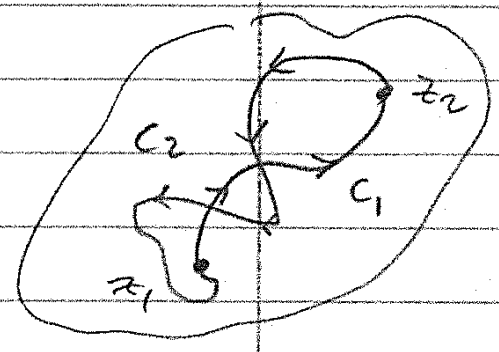
\includegraphics[scale=0.25]{c1c2}
	\end{figure}

	Note that by reversing the direction of $C_2$, we ave both $C_1$ and $-C_2$ go from $z_1$ to $z_2$ and stay inside of $\mathcal{D}$. Thus, 
	\begin{align}
	\oint_{C}f\,dz = \int_{C_1} f\,dz - \int_{-C_2}f\,dz.
	\end{align}
	By (2), we have that
	\begin{align}
	\int_{C_1} f\,dz = \int_{C_2}f\,dz.
	\end{align}
	This means 
	\begin{align}
	\oint_C f(z)\,dz = 0.
	\end{align}
	So $(2) \implies (3)$.\\
	
	Now, assume (3) is true and let $z_0, z_1 \in \mathcal{D}$. Let $C_1, C_2 \subset \mathcal{D}$ be contours going from $z_0$ to $z_1$. We observe that $C:= C_1 - C_2$ is a s.c.c. in $\mathcal{D}$. So by (3),
	\begin{align}
	0 = \oint_C f\,dz = \int_{C_1 - C_2}f\,dz = \int_{C_1} f\,dz - \int_{C_2}f\,dz.
	\end{align}	
	
	
	
	
	
	\begin{figure}[!htb]
		\centering
		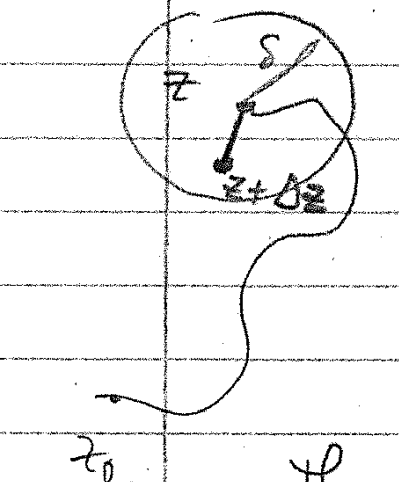
\includegraphics[scale=0.25]{tfae}
	\end{figure}
	
	
	($1\iff 2$) Assume (1) is true. Let $z_0, z_1 \in \mathcal{D}$ and let $C$ be a contour from $z_0 \to z_1$, i.e., $C: z(t) \in C([a,b],\C)$ piecewise differentiable, $z(a) = z_0$ and $z(b)= z_1$. As $F$ is an antiderivative of $f$, for all $t\in [a,b]$ for which $z'(t)$ exists the chain rule gives 
	\begin{align}
	\f{d}{dt}F(z(t)) = F'(z(t))z'(t) = f(z(t))z'(t).
	\end{align}
	So,
	\begin{align}
	\oint_C f\,dz = \sum^n_{k=1}\int^{b_k}_{a_k}f(z(t))z'(t)\,dt = \sum^n_{k=1}\int^{b_k}_{a_k} \f{d}{dt}F(z(t))\,dt
	\end{align}
	where $a_k ,b_k$ are points at which $z$ fails to be differentiable, $a_1 = a, b_n = b$. By the fundamental theorem of calculus,
	\begin{align}
	\oint_C f\,dz &=\sum^n_{k=1}\int^{b_k}_{a_k} \f{d}{dt}F(z(t))\,dt\nn\\
	&= \sum^n_{k=1}F(z(b_k)) - F(z(a_k)) \nn\\
	&= F(b) - F(a) = F(z_1) - F(z_0).
	\end{align}
	So, given any 2 contours $C_1, C_2 \in \subset \mathcal{D}$ from $z_0 \to z_1$, we have
	\begin{align}
	\int_{C_1}f\,dz = F(z_1) - F(z_0) = \int_{C_2}f\,dz.
	\end{align}
	
	
	Now, assume (2) is true. We need to construct an antiderivative $F$. Let $z_0 \in \mathcal{D}$ and define $F: \mathcal{D} \to \C$ by
	\begin{align}
	F(z) = \int_{C_z}f(w)\,dw
	\end{align}
	where $C_z$ is a contour  from $z_0 \to z_1$. Since $\mathcal{D}$ is a domain, it is a path connected, and so for each $z$, a path $C_z$ exists. By (2) this is not dependent on the choice of contour $C_z$. So $F$ is well-defined. We wish to show that $F(z)$ is differentiable and its derivative is $f$. \\
	
	Let $z \in \subset \mathcal{D}$ and choose $\epsilon > 0$. Given th continuity of $f$, let $\delta$ be chosen so that 
	\begin{enumerate}
		\item \begin{align}
		\abs{f(w) - f(z)} < \f{\epsilon}{2} \forall \abs{w-z} < \delta
		\end{align}
		
		\item $\B_\delta(z) \subset \mathcal{D}$ (or $\mathcal{D}$ is open.)
	\end{enumerate}
	
	Given a $\Delta z \in \C$ such that $\Delta z < \delta$, we consider a path $C_{z,\Delta z}$ defined by $w(t) = z + t\Delta z$, $t \in  [0,1]$. We have that $C_z + C_{z,\Delta z}$ is a contour in $\mathcal{D}$ from $z_0 \to z + \Delta z$. Then,
	\begin{align}
	\f{1}{\Delta z} \lp F(z+ \Delta z) - F(z) \rp &= \f{1}{\Delta z}\lp \int_{C_z + C_{z,\Delta z}} f(w)\,dw - \int_{C_z}f(w)\,dw \rp\nn\\
	&= \f{1}{\Delta z}\int_{C_{z,\Delta z}} f(w)\,dw\nn\\
	&= \f{1}{\Delta z}\int^1_0 f(z+t\Delta z)(z + t\Delta z)'\,dt\nn\\
	&= \int^1_0 f(z+t\Delta z)\,dt.
	\end{align}
	So, for $\abs{\Delta z} < \delta$,
	\begin{align}
	\abs{\f{F(z+\Delta z) - F(z)}{\Delta z} - f(z)} &= \abs{ \int^1_0 f(z+t\Delta z)\,dt - f(z)}\nn\\
	&= \abs{\int^1_0 \lb f(z+t\Delta z) - f(z)  \rb\,dt }\nn\\
	&\leq \int^1_0 \abs{f(z+t\Delta z) - f(z)}\,dt\nn\\
	&\leq \int^1_0 \f{\epsilon}{2}\,dt\nn\\
	&\leq \f{\epsilon}{2}\nn\\
	&< \epsilon
	\end{align}
	by choice of $\delta$. So, we have shown that given $z\in \mathcal{D}$ and $\epsilon > 0$, there exists $\delta > 0$ such that
	\begin{align}
	\abs{\f{F(z + \Delta z) - F(z)}{\Delta z} - f(z)} < \epsilon
	\end{align}
	whenever $\abs{\Delta z} < \delta$. So, $F$ is differentiable at $z$ and $F'(z) = f(z)$.
\end{proof} 


\section{Cauchy-Goursat Theorem}


Suppose that $C$ is a simple closed contour and $f$ is analytic on the interior of C and all points of $C$ then 
\begin{align}
\oint_C f(z)\,dz  =0.
\end{align}

\begin{proof}
	The proof involves slicing the interior of $C$ into squares and partial squares. I won't try to reproduce it here. 
\end{proof}



\section{Simply-connected domain}

A domain $\mathcal{D}$ is called simply-connected if every simple closed contour $C \subset \mathcal{D}$  contains only points of $\mathcal{D}$ and its interior, i.e., every simple closed contour is contractible to a point.

\section{Multiply-connected domain}

A multiply-connected domain $\mathcal{D}$ is a dmain which is not simply-connected. (very imaginative)



\section{Cauchy-Goursat Theorem for simply-connected domain}

Let $\mathcal{D}$ be a simply connected domain. $f$ is analytic in $\mathcal{D}$. For all closed contour $C \subset \mathcal{D}$,
\begin{align}
\oint_C f(z)\,dz = 0.
\end{align}

\begin{proof}
	Notice that we $C$ need not be simple. Consider the figure

	\begin{figure}[!htb]
		\centering
		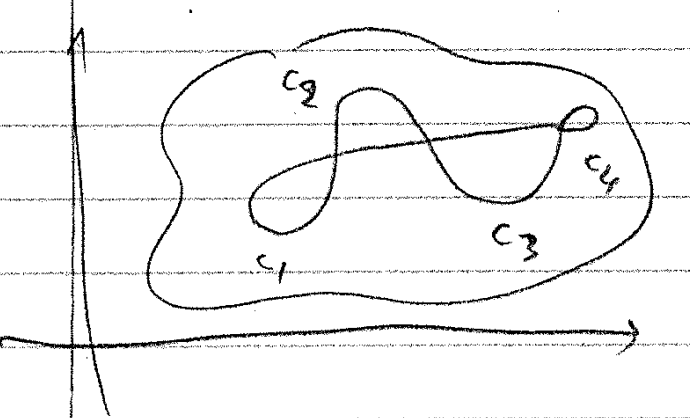
\includegraphics[scale=0.25]{C-G-simple}
	\end{figure}


	Let $C$ be a closed contour in $\mathcal{D}$ with a finite number of self-intersections. Given that $C$ only has $n$ interactions, we can split $C$ into a finite number $m$ of simple closed contour $C_j$. Also, given $\mathcal{D}$ is simply connected, the interior of each $C_j$ lives in $\mathcal{D}$. By the previous theorem, we have 
	\begin{align}
	\oint_{C_j}f(z)\,dz = 0 \forall j = 1,2,3,\dots \implies \oint_C f(z)\,dz = \oint_{\sum C_j}f(z)\,dz  = 0.
	\end{align}

\end{proof}


\section{Corollary to Cauchy-Goursat for simply-connected domain}

If $f$ is analytic on a simply connected domain in $\mathcal{D}$ then $f$ has an antiderivative $F$ everywhere in $\mathcal{D}$.

\begin{proof}
	TFAE.
\end{proof}

\section{Cauchy-Goursat Theorem for multiply-connected regions}

Suppose that
\begin{enumerate}
	\item $C$ is a s.c.c.(+).
	\item $C_j$, $j=1,2,\dots,n$ are s.c.c.(-), all disjoint and all live in the interior of $C$.
\end{enumerate}
If $f$ is analytic on $C,C_j \forall j$ and the region between $C, C_j$ (enclosed by $C$ but outside of $C_j$) then 
\begin{align}
\oint_C f(z)\,dz + \sum^n_{j=1}\oint_{C_j}f(z)\,dz = 0.
\end{align}

\begin{proof}
	The proof follows from the this figure
	\begin{figure}[!htb]
		\centering
		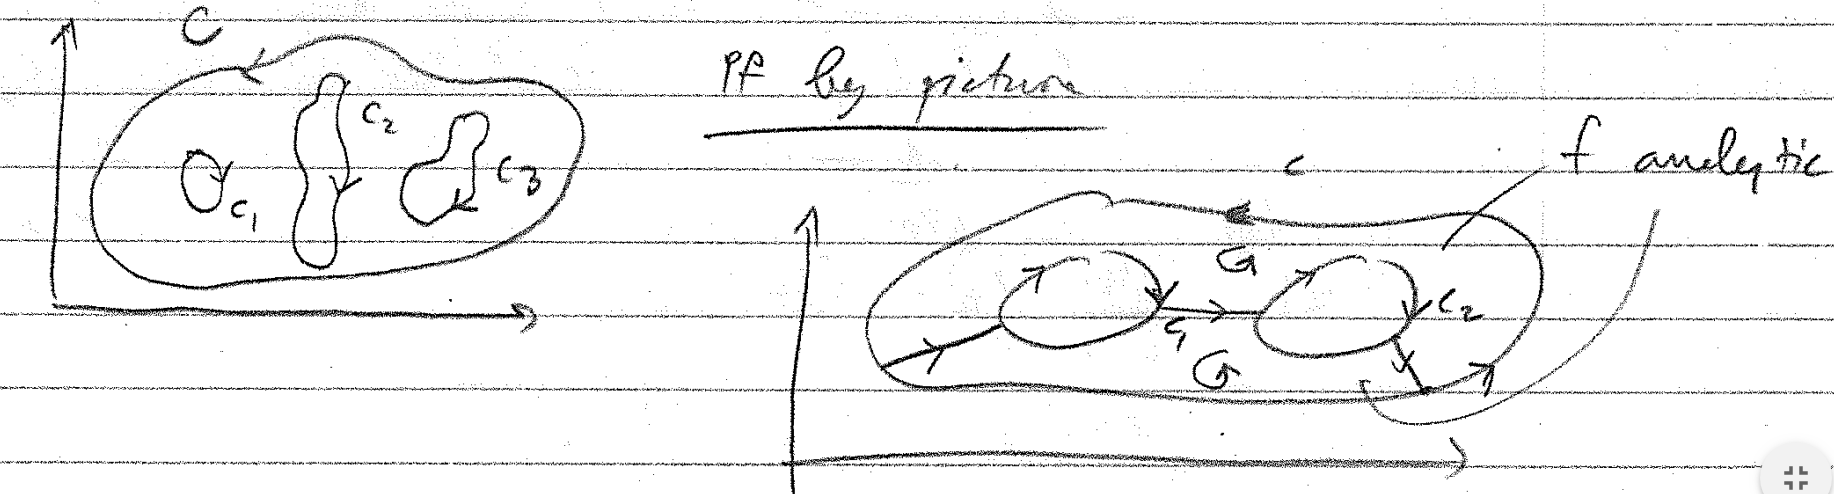
\includegraphics[scale=0.25]{C-G-multi}
	\end{figure}


\end{proof}






\section{Principle of Path Deformation (Corollary to Cauchy-Goursat)}


Let $C_1$ and $C_2$ be simple closed curves and $C_2$ encloses $C_1$. Both are (+) oriented. Then if $f$ is analytic on the region between $C_1, C_2$ then
\begin{align}
\int_{C_1}f(z)\,dz = \int_{C_2}f(z)\,dz.
\end{align}

\begin{proof}
	Consider the following suggestive figure:
	
	
	\begin{figure}[!htb]
		\centering
		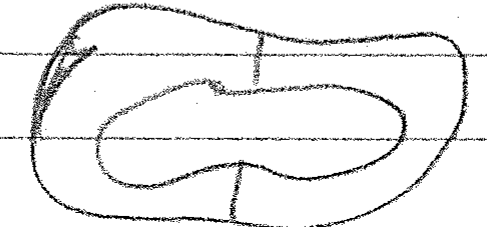
\includegraphics[scale=0.25]{deform}
	\end{figure}\qedhere
\end{proof}



\section{Cauchy's Integral Formula}

Let $C$ be a s.c.c.(+) and let $f$ be analytic on $C$ and its interior. If $z_0$ lives interior to $C$ then 
\begin{align}
f(z_0) = \f{1}{2\pi i}\oint_C \f{f(z)}{z-z_0}\,dz.
\end{align}

\begin{proof}
	\begin{figure}[!htb]
		\centering
		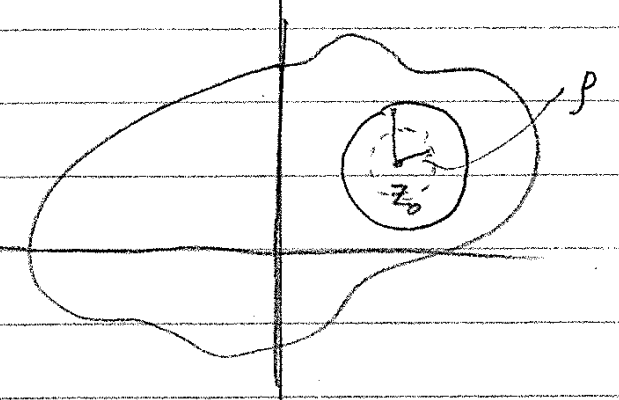
\includegraphics[scale=0.25]{cauchy1}
	\end{figure}

	Let $\delta < 1$ be small enough such that $\abs{z-z_0} < \delta$ so that $C$ encloses $z$. Since the quotient $f(z) / (z-z_0)$ is analytic in the region exterior to $\B_\delta(z_0)$ and interior to $C$, we have that
	\begin{align}
	\oint_C \f{f(z)}{z-z_0}\,dz = \oint_{C_\rho}\f{f(z)}{z-z_0}\,dz
	\end{align}
	where $\rho < \delta$ and $C_\rho$ is a (+) circle centered at $z_0$ of radius $\rho$. The equality is guaranteed by the principle of deformation of path. \\
	
	Now, consider
	\begin{align}
	\E &= \f{1}{2\pi i}\oint_C \f{f(z)}{z-z_0} - f(z_0)\nn\\
	&=\f{1}{2\pi i}\oint_{C_\rho} \f{f(z)}{z-z_0} - \f{f(z_0)}{2\pi i}\oint_{C_\rho}\f{1}{z-z_0}\,dz\nn\\
	&= \f{1}{2\pi i}\lp \oint_{C_\rho}\f{f(z) - f(z_0)}{z - z_0} \,dz\rp.
	\end{align}
	Given that $f(z)$ is continuous at $z_0$, $\forall \epsilon > 0, \exists \rho > 0 $ s.t. $\abs{f(z) - f(z_0)} < \epsilon$ whenever $\abs{z - z_0} < 2\rho < \delta$. Since $\abs{z - z_0} = \rho < 2\rho $ on $C_\rho$, we have
	\begin{align}
	\abs{\f{f(z) - f(z_0)}{z - z_0}} = \f{1}{\rho}\abs{f(z) - f(z_0)} < \f{\epsilon}{\rho} \text{ on } C_\rho.
	\end{align}
	So, 
	\begin{align}
	\abs{\E} \leq \f{1}{2\pi}\f{\epsilon}{\rho}\lag(C_\rho) = \epsilon.
	\end{align}
	So, given any $\epsilon > 0$, $\abs{\E} \leq \epsilon$. This says that 
	\begin{align}
	\f{1}{2\pi i}\oint_C \f{f(z)}{z - z_0} \,dz = f(z_0).
	\end{align}
\end{proof}



\section{Cauchy's Integral Formula for First-Order Derivative}
Let $C$ s.c.c.(+) and let $f$ be analytic on the interior of $C$ and on $C$. Then if $z_0 \in \text{int}(C)$ then 
\begin{align}
f'(z_0) = \f{1}{2\pi i}\oint_{C}\f{f(z)}{(z - z_0)^2}\,dz.
\end{align}
\begin{proof}
	\begin{figure}[!htb]
		\centering
		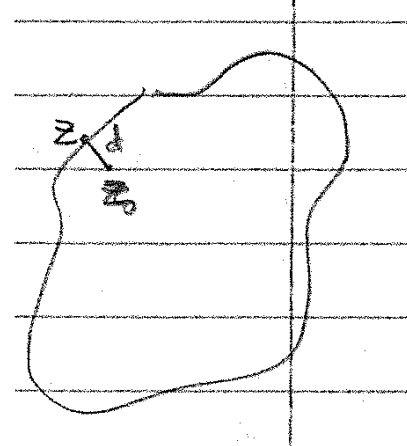
\includegraphics[scale=0.25]{cauchy2}
	\end{figure}
	
	Let $M = \max\abs{f(z)}$ where $z\in C$. Given $z_0 \in \text{int}(C)$, let $d = \min\abs{z - z_0} > 0$ where $z\in C$. Let $h = \Delta z$ is such that $\abs{h} = \abs{\Delta z} < d$. Using Cauchy's integral formula,
	\begin{align}
	f(z_0) = \f{1}{2\pi i}\oint_C \f{f(z)}{z-z_0}\,dz.
	\end{align}
	Because $\abs{h} < d$, $z_0 + h \in \text{int}(C)$. So,
	\begin{align}
	f(z_0 + h) = \f{1}{2\pi i}\oint_C \f{f(z)}{z - (z_0 + h)}\,dz.
	\end{align}
	Now, observe that
	\begin{align}
	\mathcal{E} &= \f{f(z_0 + h ) - f(z_0)}{h} - \f{1}{2\pi i}\oint_C \f{f(z)}{(z - z_0)^2}\,dz\nn\\
	&= \f{1}{h}\f{1}{2\pi i}\oint_C \f{f(z)}{z - (z_0 + h)}\,dz - \f{1}{h} \f{1}{2\pi i}\oint_C \f{f(z)}{z-z_0}\,dz- \f{1}{2\pi i}\oint_C \f{f(z)}{(z - z_0)^2}\,dz\nn\\
	&= \dots\nn\\
	&= \f{1}{2\pi i}\oint_C \f{f(z)}{(z - z_0)^2}\f{h}{z - (z_0 + h)}\,dz
	\end{align}
	for all $z \in \text{int}(C), d \leq \abs{z-z_0}$. So, 
	\begin{align}
	\f{1}{\abs{z - z_0}^2} \leq \f{1}{d^2}.
	\end{align}\
	Also, $0 \leq d - \abs{h} \leq \abs{z - (z_0 + h)}\forall \abs{h} < d$. So for all $z\in C$, whenever $\abs{h} < d$,
	\begin{align}
	\abs{\f{f(z)}{(z - z_0)^2}\f{h}{z - (z_0 + h)}} \leq \f{M\abs{h}}{d^2 (d - \abs{h})}.
	\end{align} 
	So, whenever $\abs{h} < d$, we have
	\begin{align}
	\abs{\mathcal{E}} \leq \f{1}{2\pi}\f{M\abs{h}}{d^2 (d - \abs{h})}\lag(C) = \f{M\abs{h}}{2\pi d^2 (d - \abs{h})}\lag(C).
	\end{align}
	Let $\epsilon > 0$ be given and choose 
	\begin{align}
	\delta = \min\lb \f{d}{2}, \f{\pi d^3}{M\lag(C)} \rb 
	\end{align}
	then whenever $\abs{h} < \delta \leq \f{d}{2} < d$,
	\begin{align}
	\f{1}{d - \abs{h}} \leq \f{1}{d/2}.
	\end{align} 
	With this,
	\begin{align}
	\mathcal{E} \leq \f{M\abs{h}}{2\pi d^3/2}\lag(C) < \f{M\lag(C)}{\pi d^3} \f{\pi d^3 \epsilon}{M\lag(C)} = \epsilon.
	\end{align}
	So,
	\begin{align}
	f'(z_0) =\lim_{h\to 0}\f{f(z_0 + h) - f(z_0)}{h} = \f{1}{2\pi i}\oint_C \f{f(z)}{(z - z_0)^2}\,dz.
	\end{align}
\end{proof}


\section{Cauchy's Integral Formula for Higher-Order Derivatives}
Let $C$ be s.c.c.(+) and $f$ analytic on $C$ and its interior. Then $\forall z_0 \in \text{int}(C)$, and $n\in \mathbb{N}$, $f$ is $n$-times differentiable at $z_0$ and 
\begin{align}
f^{(n)}(z_0) = \f{n!}{2\pi i}\oint_C \f{f(z)}{(z - z_0)^{n+1}}\,dz.
\end{align}



\section{Analyticity of Derivatives}

If $f$ is analytic at $z_0$ then $f$ has derivatives of all orders which are also analytic at $z_0$.

\begin{proof}
	We simply applying the preceding theorem.
\end{proof}

\section{Analyticity of Derivatives on a Domain}

If $\mathcal{D}$ is a domain and $f$ is analytic on $\mathcal{D}$ then $f$ has derivatives of all orders and each derivative is analytic on $\mathcal{D}$. This means $f$ is infinitely differentiable on $\mathcal{D}$. 


\section{Infinite Differentiability}

Let $f(z) = u(x,y) + iv(x,y)$ be analytic at $z_0 = (x_0, y_0)$. Then $u,v$ have continuous partial derivatives of all orders at $z_0$. Further, if $f = u+iv$ is analytic on $\mathcal{D}$, then $u,v$ are infinitely differentiable in $\mathcal{D}$, i.e., $u,v \in C^\infty(\mathcal{D})$.

\begin{proof}
	The proof follows from Cauchy-Riemann theorem and equations.
\end{proof}






\section{H\"{o}rmander's Theorem}

If $u$ is harmonic in a domain $\mathcal{D}$ then $u$ is smooth $\iff$ $u \in C^\infty (\mathcal{D})$.

\begin{proof}
	If $u$ is harmonic then $u$ has a harmonic conjugate $v$. Then $f = u + iv$ is analytic, etc. 
\end{proof}

\section{Morera's Theorem}

Let $f$ be continuous on $\mathcal{D}$. If for all closed $C \subset \mathcal{D}$, 
\begin{align}
\oint_C f(z)\,dz = 0,
\end{align}
then $f$ is analytic on $\mathcal{D}$. 

\begin{proof}
	The proof follows from TFAE. By TFAE, $f$ has an antiderivative $F$ throughout $\mathcal{D}$. But $F$ is analytic because $f' = F$. This means $F$'s derivatives are analytic throughout $\mathcal{D}$ as well. So, $f$ is analytic throughout $\mathcal{D}$. 
\end{proof}



\section{Cauchy's Inequality}

Let $f$ be analytic on and inside a (+) circle $C$ with center $z_0$ and radius $R$. Let $M_R = \max\lb \abs{f(z)} \rb, z\in C_R$. Then $\forall n \in \mathbb{N}$, 
\begin{align}
\abs{f^{(n)}(z_0)} \leq \f{n!M_R}{R^n}.
\end{align}


\begin{proof}
	This follows from Cauchy's integral formula and the triangle inequality:
	\begin{align}
	\abs{f^{(n)}(z_0)} &= \abs{\f{n!}{2\pi i}\oint_{C_R}  \f{f(z)}{(z - z_0)^{n+1}} \,dz}\nn\\
	&\leq \f{n!}{2\pi} \f{M_R}{R^{n+1}} (2\pi R)\nn\\
	&= \f{n! M_R}{R^n}.
	\end{align}
\end{proof}


\section{Liouville's Theorem}

If $f$ is bounded and entire and $f$ is constant. 

\begin{proof}
	Let $M \geq 0$ for which $\abs{f(z)} \leq M \forall z \in \C$. Given any $z_0 \in \C$, $f$ is analytic on every neighborhood of $z_0$ and so $\forall R > 0$,
	\begin{align}
	\abs{f'(z_0)} \leq \f{1! M_R}{R}
	\end{align}
	where $M_R = \max \abs{f(z)} \leq M$ where $z \in C_R(z_0)$. So, for any $z_0 \in \C$, $R > 0$,
	\begin{align}
	\abs{f'(z_0)} \leq \f{M}{R}.
	\end{align}
	This shows $f'(z_0) = 0 \forall z_0 \in \C$. So, $f$ is constant because $\C$ is a domain.  
\end{proof}



\section{The Fundamental Theorem of Algebra}

If $P(z)$ is a non constant polynomial, i.e., 
\begin{align}
P(z) = a_0 + a_1z^1 + \dots + a_n z^n
\end{align}
where $a_n \neq 0, n = \deg(P)$, then $\exists z_0 \in \C$ at which $P(z_0) = 0$. 




\begin{proof}
	Let 
	\begin{align}
	w = \f{a_0}{z^n} + \f{a_1}{z^{n-1}} + \dots + \f{a_{n-1}}{z}
	\end{align}
	and note that
	\begin{align}
	P(z) = (w+ a_n)z^n.
	\end{align}
	We observe that $z^k$ from $k \in \{1,2,3,\dots\}$ has $1/z^k \to 0$ has $z\to \infty$. So, given $\epsilon = \abs{a_n}/2$, there exists $R > 0$ for which
	\begin{align}
	\abs{w} \leq \f{\abs{a_n}}{2} \forall \abs{z} > R.
	\end{align}
	So, for $\abs{z} > R$, 
	\begin{align}
	\abs{w+a_n} \geq \abs{\abs{w} - \abs{a_n}} = \abs{a_n}- \abs{w} \geq \f{\abs{a_n}}{2}.
	\end{align}
	So, 
	\begin{align}
	\abs{\f{1}{P(z)}} = \f{1}{\abs{w+a_n}\abs{z^n}} \leq \f{2}{\abs{a_n}}\f{1}{\abs{z^n}} \leq \f{2}{\abs{a_n}}\f{1}{R^n}
	\end{align}
	where $\abs{z} >R$. Now, suppose that $P(z) \neq 0 \forall z \in \C$ to get a contradiction. Since $P(z)$ is never vanishes, $f(z) = 1/P(z)$ is entire. Since, in particular, $f(z)$ is continuous, it is bounded on all closed bounded set. So, $\exists M > 0$ such that $\abs{f(z)} \leq M \forall z, \abs{z} \leq R$. So, by what we've just shown
	\begin{align}
	\abs{\f{1}{P(z)}} \leq \max\lb M, \f{2}{\abs{a_n} R^n} \rb.
	\end{align} 
	So, we have $f(z)$ is bounded and entire. By Liouville's theorem, $1/P(z)$ must be constant. This is a contradiction. 
\end{proof}





\section{Corollary to The Fundamental Theorem of Algebra}

If $P(z)$ has degree $n$, then there exists $c \in \C$ and $z_1, z_2, \dots, z_n \in \C$ such that
\begin{align}
P(z) = c(z-z_1)\dots (z - z_n).
\end{align}



\section{The Maximum Modulus Principle 1}

Suppose that an analytic function $f$ has $\abs{f(z)}$ maximized at $z_0$ in some nbh $\B_\epsilon(z_0)$ for some $\epsilon > 0$. Then $f(z)$ is constant on $\B_\epsilon(z_0)$.

\begin{proof}
	Take $0 < \rho < \epsilon$ and by invoking Cauchy's integral formula, we have
	\begin{align}
	f(z_0) &=  \f{1}{2\pi i}\oint_{C_\rho} \f{f(z)}{z-z_0}\,dz\nn\\
	&= \f{1}{2\pi i}\int^{2\pi}_0 \f{f(z_0 + \rho e^{it})}{z_0 + \rho e^{it}-z_0}i\rho e^{it}\,dt\nn\\
	&= \f{1}{2\pi}\int^{2\pi}_0 f(z_0 + \rho e^{it})\,dt.
	\end{align}
	So
	\begin{align}
	\abs{f(z_0)} &= \f{1}{2\pi}\abs{\int^{2\pi}_0  f(z_0 + \rho e^{it})\,dt  }\nn\\
	&\leq \f{1}{2\pi}\int^{2\pi}_0 \underbrace{\abs{f(z_0 + \rho e^{it})}}_{\leq \abs{f(z_0)}}\,dt\nn\\
	&\leq \f{1}{2\pi }\int^{2\pi}_0 \abs{f(z_0)}\,dt = \abs{f(z_0)}.
	\end{align}
	This says 
	\begin{align}
	\abs{f(z_0)} = \f{1}{2\pi}\int^{2\pi}_0 \abs{f(z_0 + \rho e^{it})}\,dt
	\end{align}
	so
	\begin{align}
	\f{1}{2\pi}\int^{2\pi}_0 \underbrace{ \abs{f(z_0)} -\abs{f(z_0 + \rho e^{it})}}_{\geq 0}\,dt.
	\end{align}
	This says $\forall t \in [0,2\pi]$ and $\forall \rho < \epsilon$ 
	\begin{align}
	\abs{f(z_0)} = \abs{f(z_0 + \rho e^{it})}.
	\end{align}
	This is true for all $\rho < \epsilon$, so $\abs{f(z)} = \abs{f(z_0)}$ for all $z \in \B_\epsilon(z_0)$.
\end{proof}



\section{The Maximum Modulus Principle 2}
Let $f$ be analytic and non-constant on a domain $\mathcal{D}$ (open and connected), then $\abs{f(z)}$ cannot be maximized in $\mathcal{D}$. 

\begin{proof}
	Assume to reach a contradiction that $f$ is maximized at $z_0 \in \mathcal{D}$. Let $z_1 \in \mathcal{D}$ be arbitrary. Then by the following figure
	
	\newpage
	
	\begin{figure}[!htb]
		\centering
		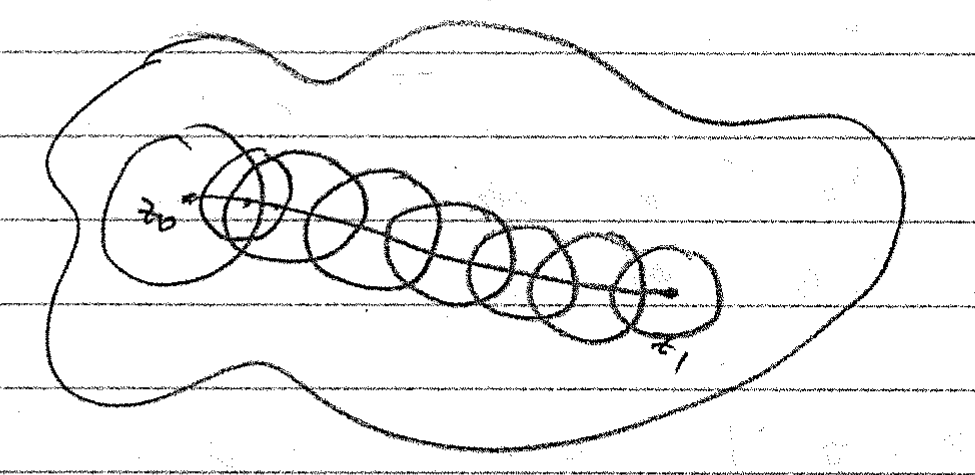
\includegraphics[scale=0.25]{max-mod}
	\end{figure}
	we get a contradiction, using the maximum modulus principle 1, as desired.  
\end{proof}




\section{Convergence of Sequences}

Consider a sequence $\{z_n\} = (z_0, z_1, \dots)$ of complex numbers. Write $\{z_n\} \in \C$. We say that the sequence converges if $\exists z \in \C$ for which the following holds: $\forall \epsilon > 0, \exists N = N_\epsilon \in \mathbb{N}$ s.t.
\begin{align}
\abs{z - z_n} < \epsilon\, \forall n \geq N.
\end{align}
In this sense, we also say that $\{z_n\}$ converges to $z$ and call $z$ the limit of the sequence:
\begin{align}
z = \lim_{n\to \infty} z_n.
\end{align}

\section{Real and Imaginary parts of a convergent sequence}
Let $z_n = x_n + iy_n$ be a sequence, then $z_n \to z = x+ iy$ if and only if $x_n \to x$ and $y_n \to y$ in the sense of real numbers. 

\section{Cauchy sequences}

A sequence $\{ z_n \}$ is called a Cauchy sequence if $\forall \epsilon > 0, \exists N \in \mathbb{N}$ such that 
\begin{align}
\abs{z_n - z_{m}} < \epsilon \,\forall n,m \geq N.
\end{align}


\section{Cauchy and Convergence}

A sequence is convergent if and only if it is Cauchy.


\section{Series}

Consider a sequence $\{z_n\}^\infty_{n=0}$ and the series formed with the sequential elements as its terms:
\begin{align}
\sum^\infty_{n=0} z_k = z_0 + z_1 + z_2 + \dots
\end{align}
where, a priori, we don't assume they add to anything. This series convergences if $\{ S_N\}$ where
\begin{align}
S_N = \sum^N_{n=0} z_k
\end{align}
is a convergent sequence, i.e.,
\begin{align}
S = \lim_{N\to \infty} S_N
\end{align}
exists. 





\section{Convergence of Series}


\noindent $\spadesuit$ Given $z_n = x_n + iy_n$ then $\sum z_n$ converges to $x + iy \iff \sum x_n \to x$ and $\sum y_n \to y$. \\

\noindent $\spadesuit$ If $\sum z_n$ converges then $\lim_{n\to \infty} z_n = 0$. The converse also holds. 

\begin{proof}
	Let $\epsilon > 0 $ be given. Then that $\sum z_n$ converges, $\{S_N\}$ also converges. So, $\{ S_N\}$ is Cauchy, so $\exists M \in \N$ such that 
	\begin{align}
	\abs{S_n - S_m} < \epsilon
	\end{align}
	whenever $n,m \geq M$. Setting $n = m+1$ we have
	\begin{align}
	\abs{z_n} = \abs{S_{n+1} - S_n} < \epsilon.
	\end{align}
\end{proof} 


\noindent $\spadesuit$ A series $\sum z_n$ is said to be absolutely convergent if $\sum \abs{z_n}$ is convergent as a series of real, non-negative numbers. \\

\noindent $\spadesuit$ If $\sum z_n$ is absolute convergent than $\sum z_n$ is convergent. 

\begin{proof}
	Here is a sketch of the proof: 
	\begin{align}
	\abs{S_N - S_M} = \abs{\sum^M_{k = N+1} z_k} \leq \sum^M_{k = N+1}\abs{z_k}
	\end{align}
	due to the triangle inequality. With this inequality, the Cauchyness of $\sum\abs{z_k}$ implies the Cauchyness of $\sum z_k$.
\end{proof}



\noindent $\spadesuit$ The series $\sum^\infty_{n=0}z_n$ converges to $S \iff \lim_{N\to \infty} \rho_N = 0$ where $\rho_N = S - S_N = S - \sum^N_{n=0}z_n$ and $S$ is some number that is to be the sum of the series. 


\noindent $\spadesuit$ ``Geometric series'':
\begin{align}
S_N = \f{1 - z^{N+1}}{1-z} = \sum^N_{n=0} z^n.
\end{align} 


\noindent $\spadesuit$ For any $z\in \C$ such that $\abs{z} < 1$, $\sum^\infty_{n=0}$ converges and its sum is $1/(1-z)$. 

\begin{proof}
	For each $N \in \N$, 
	\begin{align}
	\rho_N = \f{1}{1-z} - \sum^N_{n=0}z^n = \f{1}{1-z} - \f{1 - z^{N+1}}{1-z} = \f{z^{N+1}}{1-z}.
	\end{align}
	Since $\abs{z} < 1$, $\lim_{N\to \infty} z^{N+1} = 0$. So, $\lim_{N \to \infty} \rho_N = 0$. So, by one of the previous theorems, we have
	\begin{align}
	\sum^\infty_{n=0} z^n = \f{1}{1-z}.
	\end{align}
\end{proof}






\section{Taylor's Theorem}

Let $f(z)$ be analytic on a disk $\B_{R_0}(z_0)$, then for any $z \in \B_{R_0}(z_0)$, 
\begin{align}
f(z) = \sum^\infty_{n=0}a_n(z - z_0)^n = \sum^\infty_{n=0} \f{f^{(n)}(z_0)}{n!}(z - z_0)^n.
\end{align} 
Remarks:
\begin{enumerate}
	\item  In particular, the series $\sum^\infty_{n=0} \f{f^{(n)}(z_0)}{n!}(z - z_0)^n$ converges. 
	
	\item The sum is $f$. 
	
	\item For real functions $h: \R \to \R$. If $h$ is differentiable on an open set containing $x_0$, it might not be twice differentiable. 
	
	\item For infinitely differentiable functions, now the series makes sense, but we might have $h$ being representable by a Taylor series that is infinitely differentiable, but not equal to its Maclaurin series. For example:
	\begin{align}
	h(x) = \begin{cases}
	e^{-1/x^2}\quad x\neq 0\\
	0 \quad x = 0
	\end{cases}.
	\end{align}
\end{enumerate}



\begin{proof}
	Without loss of generality, assume that $z_0 = 0$ and consider $\B_{R_0}(z_0)$ on which $f$ is analytic. Let $z \in \B_{R_0}(z_0)$. Let $\abs{z_0} < \abs{z} < R_0$, and define a s.c.c.(+) $C$ centered at $z_0 = 0$ of radius $R_0$. Since $z$ lives in the interior of $C$, Cauchy integral formula says
	\begin{align}
	f(z) = \f{1}{2\pi i}\oint_C \f{f(w)}{w-z}\,dw.
	\end{align}
	Since $w \neq 0$, we write
	\begin{align}
	\f{1}{w-z} = \f{1}{w}\f{1}{1 - z/w} = \sum^N_{n=0}\f{z^n}{w^{n+1}} + \f{1}{w-z}\lp\f{z}{w}\rp^{N+1},
	\end{align}
	which is made possible by the fact that
	\begin{align}
	\f{1}{1-a} = \f{1 - a^{N+1}}{1 - a} + \f{a^{N+1}}{1-a} = \sum^N_{n=0}a^n + \f{a^{N+1}}{1-a}.
	\end{align}
	Next, by Cauchy's derivative formula,
	\begin{align}
	f^{(n)}(0) = \f{n!}{2\pi i}\oint_{C}\f{f(w)}{(w - 0)^{n+1}}\,dw.
	\end{align}
	So we have
	\begin{align}
	a_n = \f{f^{(n)}(0)}{n!} = \f{1}{2\pi i}\oint_{C}\f{f(w)}{(w - 0)^{n+1}}\,dw.
	\end{align}
	Next, let the error be
	\begin{align}
	\rho_N  &= f(z) -  \sum^N_{n=0} a_nz^n \nn\\
	&= \f{1}{2\pi i}\oint_C \f{f(w)}{w-z}\,dw  -  \sum^N_{n=0}\f{f^{(n)}(0)}{n!} = \f{1}{2\pi i}\oint_{C}\f{f(w)}{(w - 0)^{n+1}}z^n\,dw \nn\\
	&= \f{1}{2\pi i}\oint_C f(w)\lb \f{1}{w-z} - \sum^N_{n=0}\f{z^n}{w^{n+1}} \rb\,dw\nn\\
	&= \f{1}{2\pi i}\oint_C f(w) \f{(z/w)^{N+1}}{w-z}\,dw.
	\end{align}
	Set 
	\begin{align}
	d = \min\abs{w-z} \quad z \in C
	\end{align}
	and
	\begin{align}
	M = \max \abs{f(z)} \quad z\in \B_{R_0}(z_0 = 0)
	\end{align}
	then 
	\begin{align}
	\abs{\rho_N} &= \f{1}{2\pi} \abs{\oint_C  f(w) \f{(z/w)^{N+1}}{w-z}\,dw} \nn\\
	&\leq \f{1}{2\pi} \f{\abs{z/w}^{N+1}}{d}M \lag(C)\nn\\
	&= \f{M \abs{z/w}^{N+1}}{d}r_0
	\end{align}
	So, we have shown that given $z\in \B_{R_0}(0)$, $\exists \abs{z} < r_0 < R_0$ for which 
	\begin{align}
	\abs{\rho_N} \leq M \f{\abs{z}^{N+1}}{d\cdot r_0^N} = \lp \f{M\abs{z}}{d} \rp\lp \f{\abs{z}}{r_0} \rp^N \forall N \in \mathbb{N}.
	\end{align}
	Since we've chosen $\abs{z} < r_0 < R_0$, $\abs{z} / r_0 < 1$. Given $\epsilon > 0$, $\exists N_0 \in \mathbb{N}$ for which $\forall N \geq N_0$, 
	\begin{align}
	\lp \f{\abs{z}}{r_0} \rp^N < \f{\epsilon d}{M \abs{z}}.
	\end{align}
	So, for all $N \geq N_0$, 
	\begin{align}
	\abs{\rho_N} \leq \f{M\abs{z}}{d}\lp \f{\abs{z}}{r_0} \rp^N < \epsilon.
	\end{align}
	Thus, 
	\begin{align}
	f(z) = \lim_{N\to \infty} S_N = \lim_{N\to \infty} \sum^N_{n=0}a_n z^n = \sum^\infty_{n=0}\f{f^{(n)}(0)}{n!}z^n.
	\end{align}
\end{proof}






\section{Laurent's Theorem}

Let $f$ be analytic on a region $\mathcal{D}$ defined by $R_1 < \abs{z - z_0} < R_2$, and let a simple closed contour $C$ endowed with a positive orientation in this annulus be given. Then, for each $z \in \mathcal{D}$, 
\begin{align}
f(z) = \sum_{n =0}^\infty a_n (z - z_0)^n + \sum_{n = 1}^\infty \f{b_n}{ (z - z_0)^{-n+1}}
\end{align}
where
\begin{align}
a_n  = \f{1}{2\pi i }\oint_C \f{f(z)}{(z - z_0)^{n+1}}\,dz \quad b_n = \f{1}{2\pi i}\oint_C \f{f(z)}{(z - z_0)^{-n+1}}\,dz.
\end{align}


\begin{proof}
	\begin{figure}[!htb]
		\centering
		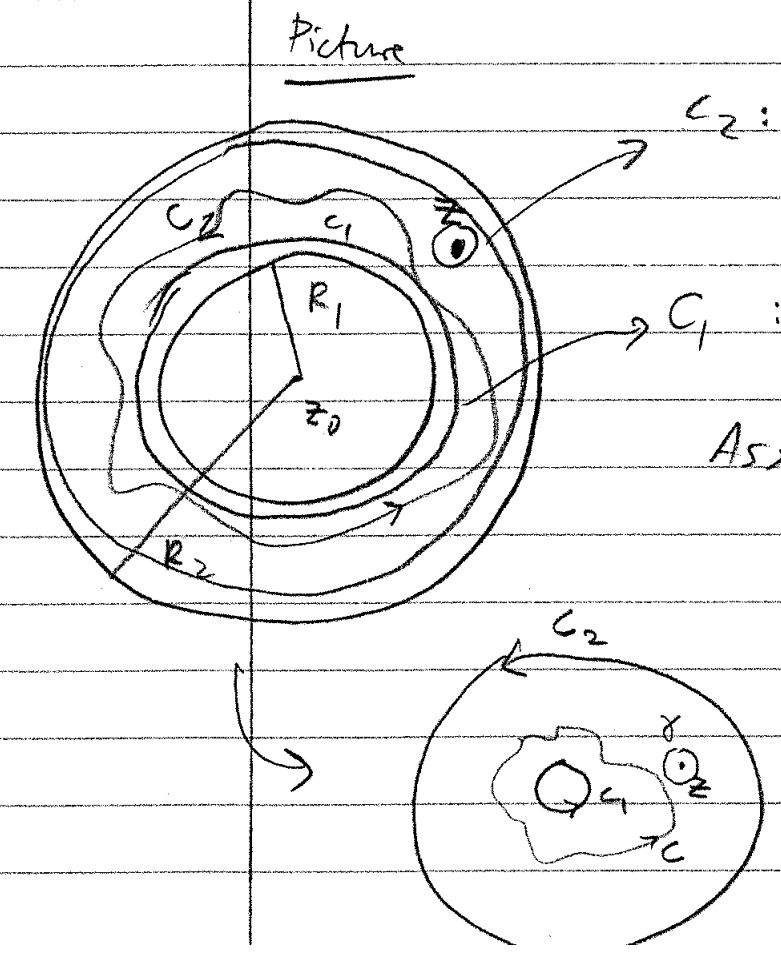
\includegraphics[scale=0.25]{laurent}
	\end{figure}
	
	Without loss of generality, assume $z_0 = 0$. Let $C_1, C_2$, s.c.c.(+) be given such that $C_2$ encloses $C_1, z, C$; $C$ encloses $C_1$, and the exterior of $C_1$ contains $z, C$. Also, let $\gamma$ be a s.c.c.(+) around $z$, exterior to $C_1$ but interior to $C_2$. An appeal to Cauchy-Goursat for multiply-connected domain shows that
	\begin{align}
	\oint_{C_2}\f{f(s)}{s-z}\,ds - \oint_{C_1}\f{f(s)}{s-z}\,ds - \oint_{C_\gamma}\f{f(s)}{s-z}\,ds = 0.
	\end{align}
	Next, by Cauchy integral formula,
	\begin{align}
	f(z) &= \f{1}{2\pi i}\oint_{C_\gamma} \f{f(s)}{s-z}\,ds \nn\\
	&= \oint_{C_2}\f{f(s)}{s-z}\,ds - \oint_{C_1}\f{f(s)}{s-z}\,ds \nn\\
	&= \oint_{C_2}\f{f(s)}{s-z}\,ds + \oint_{C_1}\f{f(s)}{z-s}\,ds.
	\end{align}
	For the first integral, we can make the following replacement
	\begin{align}
	\f{1}{s-z} &= \f{1}{s}\lp \f{1}{1 - z/s} \rp \nn\\
	&= \sum^{N-1}_{n=0} \f{z^n}{s^{n+1}} + \f{1}{s-z}\lp\f{z}{s}\rp^N.
	\end{align}
	For the second integral, we can make the following replacement (interchanging the role of $s$ and $z$)
	\begin{align}
	\f{1}{z-s} &= \f{1}{z}\lp \f{1}{1 - s/z} \rp \nn\\
	&= \sum^{N-1}_{n=0} \f{s^n}{z^{n+1}} + \f{1}{z-s}\lp\f{s}{z}\rp^N\nn\\
	&= \sum^{N}_{n=1} \f{s^{n-1}}{z^{n}} + \f{1}{z-s}\lp\f{s}{z}\rp^N\nn\\
	&= \sum^N_{n=1}\f{z^{-n}}{s^{-n+1}} + \f{1}{z-s}\lp \f{s}{z} \rp^N.
	\end{align}
	And so we have
	\begin{align}
	f(z) &= \f{1}{2\pi i}\oint_{C_2}f(s)\lb \sum^{N-1}_{n=0} \f{z^n}{s^{n+1}} + \f{1}{s-z}\lp\f{z}{s}\rp^N  \rb z^n\,dz\nn\\
	 &+ \f{1}{2\pi i}\oint_{C_1}f(s)\lb \sum^N_{n=1}\f{z^{-n}}{s^{-n+1}} + \f{1}{z-s}\lp \f{s}{z} \rp^N \rb z^{-n}\,dz \nn\\
	 &= \sum^{N-1}_{n=0}\underbrace{\lb \f{1}{2\pi i}\oint_{C_2}\f{f(s)}{s^{n+1}}\,ds \rb}_{\alpha_n} z^n + \sum^N_{n=1}\underbrace{\lb \f{1}{2\pi i} \oint_{C_1}\f{f(s)}{s^{-n+1}}\,ds\rb}_{\beta_n} z^{-n} + \rho_N + \sigma_N
	\end{align}
	where
	\begin{align}
	\rho_N = \f{1}{2\pi i}\oint_{C_2} \f{f(s)}{s-z}\lp \f{z}{s} \rp^N\,ds\\
	\sigma_N = \f{1}{2\pi i}\oint_{C_1} \f{f(s)}{z-s}\lp \f{s}{z} \rp^N\,ds.
	\end{align}
	Now, on $C_2$,
	\begin{align}
	\f{1}{\abs{s-z}} \leq \f{1}{R_2 - R},
	\end{align}
	and on $C_1$, 
	\begin{align}
	\f{1}{\abs{z-s}} \leq \f{1}{R - R_1},
	\end{align}
	where $R = \abs{z}$, $R_1< R <R_2$. Setting $M = \max\abs{f(s)}$ where $s \in C_1 \cap C_2$, by triangle inequality, we have that
	\begin{align}
	\abs{\rho_N} = \f{1}{2\pi} \abs{\oint_{C_2}\f{f(s)}{s-z}\lp \f{z}{s} \rp^N\,ds} \leq \f{1}{2\pi }\f{M}{R_2 - R}\lp \f{R}{R_2} \rp^N 2\pi R_2 = \f{M}{1 - R/R_2}\lp \f{R}{R_2} \rp^N.
	\end{align}
	Similarly,
	\begin{align}
	\abs{\sigma_N} \leq \f{M}{1 - R_1/R}\lp \f{R_1}{R} \rp^N.
	\end{align}
	We see that $\rho_N \to 0$, $\sigma \to 0$ as $N \to \infty$. It follows (with $\epsilon$'s and $N$'s similar to those in the proof of Taylor's theorem) that
	\begin{align}
	f(z) = \sum^\infty_{n=0}\alpha_n z^n + \sum^\infty_{n=1} \beta_n z^{-n}.
	\end{align}
	And by corollary to Cauchy-Goursat for multiply-connected regions, 
	\begin{align}
	\alpha_n = \f{1}{2\pi i}\int_C (\,\,\,) \,ds = a_n\nn\\
	\beta_n = \f{1}{2\pi i}\int_C (\,\,\,) \,ds = b_n
	\end{align}
	for all $n$. 
\end{proof}



\section{More results about series}
Consider a power series 
\begin{align}
S(z) = \sum^\infty_{n=0} a_n (z - z_0)^n,
\end{align}
\begin{enumerate}
	\item If $S(z)$ converges at some $z_1 \neq z_0$ the $S(z)$ converges on $\B_R(z_0)$ where $\abs{z_0 - z_1} \leq R$. 
	
	\item The series converges uniformly and absolutely on every ball $\B$ properly contained in $\B_R(z_0)$.
	
	\item On $\B_R(z_0)$, $S(z)$ is analytic, $S'(z) = \sum^\infty_{n=1} n a_n(z - z_0)^{n-1}$. 
	
	\item If $C$ is a s.c.c.(+) and $g$ is continuous on $C$ and $C \subset \B_R(z_0)$ then
	\begin{align}
	\oint_C fg\,dz = \sum^\infty_{n=0} \oint_C a_n g(z)(z - z_0)^n\,dz
	\end{align}
	
	\item Uniqueness of Laurent series: If $S(z)= \sum_{n \in \mathbb{Z}} c_n (z - z_0)^n$ converges on an annulus $R_1 \leq \abs{z - z_0} \leq R_2$ then this is precisely the Laurent series of $S$ at $z_0$. 
\end{enumerate}


\section{Residues}
For $C$ a s.c.c.(+), let $f$ have singularities at $z_1, z_2,\dots,z_n$ enclosed by $C$. Then all the $z_k$'s are isolated singularities, and there exist punctured disks $\B_1, \B_2, \dots, \B_n$ inside $C$ which are on-overlapping whose centers contains $z_k$'s, respectively.\\

Next, suppose that $f$ has an isolated singularity at $z_0$. Then $f$ has a Laurent series expansion on an annulus $0 < \abs{z-z_0} < R$ with
\begin{align}
f(z) = \sum^\infty_{n=0}a_n (z - z_0)^n + \sum^\infty_{n=1}\f{b_n}{(z - z_0)^n}.
\end{align}
Further, for any s.c.c.(+) $C_k$,
\begin{align}
b_n = \f{1}{2\pi i} \oint_{C_k} \f{f(z)}{(z - z_0)^{-n+1}}\,dz \forall n = 1,2,3,\dots
\end{align}
In particular, 
\begin{align}
b_1 = \f{1}{2\pi i}\oint_{C_k} f(z)\,dz.
\end{align}
We shall call this coefficient of $1/ (z - z_0)$ in the Laurent series expansion the residue of $f$ at $z_0$, denoted
\begin{align}
b_1 := \Res_{z = z_0} f(z).
\end{align}
This gives us a way to compute integrals by finding Laurent series expansions.

\section{The Residue Theorem}

Let $C$ be a s.c.c.(+) and suppose that $f$ is analytic on $C$ and the interior to $C$ except at a finite number of points $z_1, z_2, \dots, z_n$, all enclosed by $C$. Then
\begin{align}
\oint_C f(z)\,dz = 2\pi i\sum^n_{k=1}\Res_{z = z_k} f(z).
\end{align}

\begin{proof}
	Take $C_1, C_2, \dots, C_n$ to be non-intersecting s.c.c.(+) inside $C$ where each enclosed only the singular point $z_k$, respectively. Then $f$ is analytic on $\text{Int}(C)\setminus \cup^n \text{Int}C_k$. By Cauchy-Goursat for multiply-connected region, 
	\begin{align}
	\oint_C f(z)\,dz = \sum^n_{k=1}\oint_{C_k} f(z)\,dz.
	\end{align}
	But for each $k$, we also have
	\begin{align}
	\oint_{C_k} f(z)\,dz = 2\pi i \Res_{z = z_k} f(z).
	\end{align}
	So,
	\begin{align}
	\oint_C f(z)\,dz = 2\pi i\sum^n_{k=1}\Res_{z = z_k} f(z).
	\end{align}\qedhere
\end{proof}



\section{Classification of Singularities}

If the principal part of the Laurent series expansion of $f$ is identically zero then $z_0$ is said to be a removable singularity. \\

If $z_0$ is an isolated removable singularity for $f$ for $z \neq z_0$ but $0 < \abs{z - z_0} < R$, then 
\begin{align}
f(z) = \sum^\infty_{n=0}a_n (z - z_0)^n+ 0 .
\end{align}
At $z = z_0$, the left-hand side is $a_0$. So if we define
\begin{align}
f_{ext}(z) = \begin{cases}
f(z) \quad 0 < \abs{z - z_0} < R\\
a_0 \quad z = z_0
\end{cases}
\end{align}
then 
\begin{align}
f_{ext}(z) = \sum^\infty_{n=0}a_n (z - z_0)^n 
\end{align}
for all $z$ such that $\abs{z - z_0} < R$. This is called an extension of $f$. We note that $f_{ext}(z)$ is analytic on $\mathcal{B}_R(z_0)$. We have just removed the removable singularity. \\

When the principal part of $f$ is nonzero and contains a finite number of summands 
\begin{align}
\sum^\infty_{n=1}\f{b_n}{(z - z_0)^n} = \f{b_1}{(z - z_0)} + \dots \f{b_m}{(z - z_0)^m}
\end{align}
and $b_k \neq 0 \forall k \geq m+1$ then $z_0$ is a pole of order $m$ for $f$. When $m=1$, $z_0$ is called a simple pole.\\

If the principal part of $f$ is identically zero, then $z_0$ is a removable singularity for $f$, because $f$ can be extended via its valid Taylor-Laurent series expansion to an analytic function on $\mathcal{B}_R(z_0)$. \\

$z_0$ is said to be an essential singularity of $f$ it it is not removable or a pole, i.e., the principle part of the Laurent series of $f$ contains an infinite number of non-zero terms.  


\section{Residues with $\Phi$ theorem}

Let $z_0$ be an isolated singularity of $f$. Then $z_0$ is a pole or order $m$ if and only if $\exists$ a function $\phi(z)$ which is non zero at $z_0$, analytic at $z_0$ and for which 
\begin{align}
f(z) = \f{\phi(z)}{(z-z_0)^m}
\end{align}
for $z \in $ a nbh of $z_0$. In this case,
\begin{align}
\Res_{z = z_0} f(z) = \f{\phi^{(m-1)}(z_0)}{(m-1)!}.
\end{align}

\begin{proof}
	($\rightarrow$) Suppose that 
	\begin{align}
	f(z) = \f{\phi(z)}{(z-z_0)^m}
	\end{align}
	where $\phi(z)$ is analytic at $z_0$ and $\phi(z_0) \neq 0$. Then we have that $\phi(z)$ has a valid Taylor series expansion in $\mathcal{B}_R(z_0)$:
	\begin{align}
	\phi(z) = \sum^\infty_{n=0} \f{\phi^{(n)}(z_0)}{n!}(z- z_0)^n.
	\end{align} 
	With this, we can write $f(z)$ as
	\begin{align}
	f(z) &= \f{1}{(z-z_0)^m} \sum^\infty_{n=0}\f{\phi^{(n)}(z_0)}{n!}(z-z_0)^n\nonumber\\
	&= \sum^\infty_{n=0}\f{\phi^{(n)}(z_0)}{n!}(z-z_0)^{n-m}\nonumber\\
	&= \sum^{m-1}_{n=0}\f{\phi^{(n)}(z_0)}{n!}(z-z_0)^{n-m} + \text{(Taylor)}\nonumber\\
	&= \sum^{m}_{k=1}\f{\phi^{(n-k)}(z_0)}{(m-k)!}(z-z_0)^{k} + \text{(Taylor)}, \quad (k= m-n).
	\end{align}
	And so $z_0$ is a pole of order $m$, since $\phi^{(0)}(z_0) \neq 0$. And of course, we get for free
	\begin{align}
	\Res_{z = z_0} f(z) = \f{\phi^{(m-1)}(z_0)}{(m-1)!}.
	\end{align}
	
 	($\leftarrow$) Conversely, assume that $f$ has a pole at $z_0$ or order $m$. Then 
 	\begin{align}
 	f(z) &= \sum^\infty_{n=0}a_n(z-z_0)^n + \sum^\infty_{n=1} \f{b_n}{(z - z_0)^n} + 0 \dots\nonumber\\
 	&= \f{1}{(z-z_0)^m}\lb \sum^\infty_{n=0}a_n(z-z_0)^{n+m} + \sum^\infty_{n=1} \f{b_n}{(z - z_0)^{n-m}}   \rb\nonumber\\
 	&:= \f{\phi(z)}{(z - z_0)^m}
 	\end{align}
 	where $\phi(z)$ is defined to be the expression in the square brackets. With this, we see that $\phi(z)$ is analytic at $z_0$ and $\phi(z_0) = 0 + b_m \neq 0 $ by hypothesis. \qedhere
\end{proof}




\section{Residues with p-q theorem}
Let $p,q$ be analytic at $z_0$. If $p(z_0) \neq 0, q'(z_0) \neq 0$, and $p'(z_0) = 0$ then
\begin{align}
f(z) = \f{p(z)}{q(z)}
\end{align}
has a simple pole of $z_0$ and 
\begin{align}
\Res_{z = z_0} f(z) =\Res_{z = z_0}\f{p(z)}{q(z)} = \f{p(z_0)}{q'(z_0)}.
\end{align}
\begin{proof}
	Since $q'(z_0) \neq 0$, $q$ has a simple zero at $z_0$. So $1/q$ has a simple pole at $z_0$ and 
	\begin{align}
	\Res_{z = z_0}\f{1}{q} = \f{1}{q'(z_0)}.
	\end{align}
	Since $p(z_0) \neq 0$, we know that
	\begin{align}
	\Res_{z=z_0}\f{p}{q} = p(z_0)\Res_{z = z_0}\f{1}{q} = \f{p(z_0)}{q'(z_0)}.
	\end{align}
\end{proof}


\begin{proof}
	This proof should be more elaborate than the previous proof: 
\end{proof}

\newpage

\section{What happens near singularities?}

If $z_0$ is a pole of order $m$ for $f$, then 
\begin{align}
\lim_{z \to z_0} f(z) = \infty.
\end{align}


\section{Removable singularity - Boundedness - Analyticity (RBA)}
If $z_0$ is a removable singularity for $f$ then $f$ is bounded and analytic on a punctured nbh of $z_0$.


\section{The converse of RBA}
Let $f$ be analytic on $0 < \abs{z-z_0} < \delta $ for some $\delta > 0$. If $f$ is also bounded on $ 0 < \abs{z-z_0} < \delta$, then if $z_0$ is a singularity for $f$, it must be removable. \\

\noindent \begin{proof}
	By assumption, $f$ has a Laurent series representation of the form
	\begin{align}
	f(z) = \sum^\infty_{n=0}a_n(z-z_0)^n + \sum^\infty_{n=1}\f{b_n}{(z-z_0)^n}  
	\end{align}
	where $b_n$ in particular is given by
	\begin{align}
	b_n = \f{1}{2\pi i}\oint_C \f{f(z)}{(z-z_0)^{-n+1}}\,dz
	\end{align}
	where $C$ is a s.c.c.(+) in the annulus of the analyticity. In particular, if $0 < \rho < \delta$, and $C_\rho := \{ z, \abs{z - z_0} = \rho \}$, (+) then
	\begin{align}
	\abs{b_n} = \abs{\f{1}{2\pi i}\oint_{C_\rho} \f{f(z)}{(z-z_0)^{-n+1}}\,dz}
	\end{align} 
	and if $M$ is such that $f(z) \leq M \forall 0 < \abs{z-z_0} < \delta$ then 
	\begin{align}
	\abs{b_n} \leq \f{1}{2\pi}\f{M}{\rho^{-n+1}}2\pi \rho = M \rho^{n}.
	\end{align}
	Since this is valid $\forall \rho < \delta$, we must have that $b_n = 0 \forall n$. \qedhere
\end{proof}


\section{Casorati-Weierstrass Theorem}

Let  $f$ have an essential singularity at $z_0$. Then $\forall w_0 \in \C$ and $\epsilon > 0$,
\begin{align}
\abs{f(z) - w_0} < \epsilon 
\end{align}
for some $z\in \mathcal{B}_\delta(z_0) \forall \delta  0$.\\
$\iff f$ is arbitrarily close to every complex number on every nbh of $z_0$.\\
$\iff \forall \delta > 0, f(\mathcal{B}_\delta(z_0)\setminus\{z_0\} )$ is dense on $\C$. \\
$\iff f$ gets close to every single point in a ball for any ball.\\
$\iff$ If $z_0$ is an essential singularity for $f$ then $f$ attains, except for at most one value, every complex number an infinite  number of time on every nbh of $z_0$.\\

\noindent \begin{proof}
	Assume to reach a contradiction that $\exists w_0 \in \C, \epsilon, \delta >0 $ s.t.
	\begin{align}
	\abs{f(z) - w_0} \geq \epsilon \forall 0 < \abs{z-z_0} < \delta,
	\end{align} 
	i.e., $f$ does not get close to some value $w_0$ in some nbh of $z_0$ of radius $\delta$. Then, consider 
	\begin{align}
	g(z) = \f{1}{f(z) - w_0}
	\end{align} 
	which is bounded and analytic on the punctured disk $0 < \abs{z-z_0} < \delta$. At worst, $z_0$ is a removable singularity for $g$. Also note that $g(z)$ is not identically zero since $f$ is not constant (as $f$ has a singularity). With this, 
	\begin{align}
	g(z) = \sum^\infty_{k=0}a_k (z-z_0)^k,
	\end{align}  
	which allows us to extend $g$ to $z_0$. Let $m = \min(k=0,1,2,\dots)$ such that $a_k \neq 0$, which exists because $g\neq 0$. Then
	\begin{align}
	g(z) = (z-z_0)^m\sum^\infty_{k=0}a_k (z-z_0)^{k-m} = (z-z_0)^m\sum^\infty_{k=0}a_{k+m} (z-z_0)^k.
	\end{align}
	Call the sum $h(z)$, which $h(z_0) = a_m \neq 0$. So, in $\B_\delta(z_0)\setminus\{z_0\}$, we have
	\begin{align}
	f(z)  =w_0 + \f{1}{g(z)}.
	\end{align}
	If $g(z_0) \neq 0 \iff m= 0$, then this formula allows s to extend $f$ to $z_0$, which is then analytic, which makes $z_0$ a removable singularity. This is a contradiction. If $g(z_0) = 0$, then because $ m\geq 1$ (by definition) and
	\begin{align}
	f(z) = w_0 + \f{1}{g(z)} = \f{w_0 g(z) + 1}{(z-z_0)^m h(z)} := \f{\phi(z)}{(z - z_0)^m}.
	\end{align} 
	We see that $\phi(z_0) \neq 0$, and $\phi(z)$ is analytic. So, $z_0$ is a pole of order $m$ of $f$. This is also a contradiction. \qedhere
	
\end{proof}
















\end{document}
